% -*- Mode:TeX -*-

%% IMPORTANT: The official thesis specifications are available at:
%%            http://libraries.mit.edu/archives/thesis-specs/
%%
%%            Please verify your thesis' formatting and copyright
%%            assignment before submission.  If you notice any
%%            discrepancies between these templates and the 
%%            MIT Libraries' specs, please let us know
%%            by e-mailing thesis@mit.edu

%% The documentclass options along with the pagestyle can be used to generate
%% a technical report, a draft copy, or a regular thesis.  You may need to
%% re-specify the pagestyle after you \include  cover.tex.  For more
%% information, see the first few lines of mitthesis.cls. 

%\documentclass[12pt,vi,twoside]{mitthesis}
%%
%%  If you want your thesis copyright to you instead of MIT, use the
%%  ``vi'' option, as above.
%%
%\documentclass[12pt,twoside,leftblank]{mitthesis}
%%
%% If you want blank pages before new chapters to be labelled ``This
%% Page Intentionally Left Blank'', use the ``leftblank'' option, as
%% above. 

\documentclass[12pt,twoside]{mitthesis}
\usepackage{lgrind}

% Math and physics packages
\usepackage{amsmath}
\usepackage{amssymb}
\usepackage{physics}
\usepackage{upgreek}
\usepackage{xcolor}

% New commands

\newcommand{\jcp}{Journal of Chemical Physics}
\newcommand{\physrep}{Physics Reports}
\newcommand{\pra}{Physical Review A}
\newcommand{\prb}{Physical Review B} 



% For hyperlinks
\usepackage{hyperref} % For hyperlinks
\usepackage{url}
\usepackage[normalem]{ulem}
%\usepackage[hyperref=true,doi=false,url=false,isbn=false,backend=bibtex,style=nature]{biblatex}
%\usepackage{abntcite}

% For images and Figures
\usepackage{graphicx}
\graphicspath{{./Images/PDFs/}} % Sets the path to the images as a subdirectory included in the same directory as the .tex file. 

%\usepackage[hyperref=true,doi=false,url=false,isbn=false,backend=bibtex,style=nature]{biblatex}

%% These have been added at the request of the MIT Libraries, because
%% some PDF conversions mess up the ligatures.  -LB, 1/22/2014
\usepackage{cmap}
\usepackage[T1]{fontenc}
\pagestyle{plain}

%% This bit allows you to either specify only the files which you wish to
%% process, or `all' to process all files which you \include.
%% Krishna Sethuraman (1990).

%\typein [\files]{Enter file names to process, (chap1,chap2 ...), or `all' to
%process all files:}
\def\all{all}
\ifx\files\all \typeout{Including all files.} \else %\typeout{Including only \files.} \includeonly{\files} \fi

\begin{document}

% -*-latex-*-
% 
% For questions, comments, concerns or complaints:
% thesis@mit.edu
% 
%
% $Log: cover.tex,v $
% Revision 1.8  2008/05/13 15:02:15  jdreed
% Degree month is June, not May.  Added note about prevdegrees.
% Arthur Smith's title updated
%
% Revision 1.7  2001/02/08 18:53:16  boojum
% changed some \newpages to \cleardoublepages
%
% Revision 1.6  1999/10/21 14:49:31  boojum
% changed comment referring to documentstyle
%
% Revision 1.5  1999/10/21 14:39:04  boojum
% *** empty log message ***
%
% Revision 1.4  1997/04/18  17:54:10  othomas
% added page numbers on abstract and cover, and made 1 abstract
% page the default rather than 2.  (anne hunter tells me this
% is the new institute standard.)
%
% Revision 1.4  1997/04/18  17:54:10  othomas
% added page numbers on abstract and cover, and made 1 abstract
% page the default rather than 2.  (anne hunter tells me this
% is the new institute standard.)
%
% Revision 1.3  93/05/17  17:06:29  starflt
% Added acknowledgements section (suggested by tompalka)
% 
% Revision 1.2  92/04/22  13:13:13  epeisach
% Fixes for 1991 course 6 requirements
% Phrase "and to grant others the right to do so" has been added to 
% permission clause
% Second copy of abstract is not counted as separate pages so numbering works
% out
% 
% Revision 1.1  92/04/22  13:08:20  epeisach

% NOTE:
% These templates make an effort to conform to the MIT Thesis specifications,
% however the specifications can change.  We recommend that you verify the
% layout of your title page with your thesis advisor and/or the MIT 
% Libraries before printing your final copy.
\title{Tunable and broadband loop gap resonator for nitrogen vacancy centers in diamond}

\author{Erik Roger Eisenach}
% If you wish to list your previous degrees on the cover page, use the 
% previous degrees command:
%       \prevdegrees{A.A., Harvard University (1985)}
% You can use the \\ command to list multiple previous degrees
%       \prevdegrees{B.S., University of California (1978) \\
%                    S.M., Massachusetts Institute of Technology (1981)}
\prevdegrees{B.S., The Citadel, The Military College of South Carolina (2015)}
\department{Department of Electrical Engineering and Computer Science}

% If the thesis is for two degrees simultaneously, list them both
% separated by \and like this:
% \degree{Doctor of Philosophy \and Master of Science}
\degree{Master of Science in Electrical Engineering and Computer Science}

% As of the 2007-08 academic year, valid degree months are September, 
% February, or June.  The default is June.
\degreemonth{June}
\degreeyear{2018}
\thesisdate{May 23, 2018}

%% By default, the thesis will be copyrighted to MIT.  If you need to copyright
%% the thesis to yourself, just specify the `vi' documentclass option.  If for
%% some reason you want to exactly specify the copyright notice text, you can
%% use the \copyrightnoticetext command.  
%\copyrightnoticetext{\copyright IBM, 1990.  Do not open till Xmas.}

% If there is more than one supervisor, use the \supervisor command
% once for each.
\supervisor{Dirk Englund}{Associate Professor, Massachusetts Institute of Technology}
\supervisor{Danielle Braje}{Assistant Group Leader, Lincoln Laboratory}

% This is the department committee chairman, not the thesis committee
% chairman.  You should replace this with your Department's Committee
% Chairman.
\chairman{Leslie A. Kolodziejski}{Chairman, Department Committee on Graduate Theses}

% Make the titlepage based on the above information.  If you need
% something special and can't use the standard form, you can specify
% the exact text of the titlepage yourself.  Put it in a titlepage
% environment and leave blank lines where you want vertical space.
% The spaces will be adjusted to fill the entire page.  The dotted
% lines for the signatures are made with the \signature command.
\maketitle

% The abstractpage environment sets up everything on the page except
% the text itself.  The title and other header material are put at the
% top of the page, and the supervisors are listed at the bottom.  A
% new page is begun both before and after.  Of course, an abstract may
% be more than one page itself.  If you need more control over the
% format of the page, you can use the abstract environment, which puts
% the word "Abstract" at the beginning and single spaces its text.

%% You can either \input (*not* \include) your abstract file, or you can put
%% the text of the abstract directly between the \begin{abstractpage} and
%% \end{abstractpage} commands.

% First copy: start a new page, and save the page number.
\cleardoublepage
% Uncomment the next line if you do NOT want a page number on your
% abstract and acknowledgments pages.
% \pagestyle{empty}
\setcounter{savepage}{\thepage}
\begin{abstractpage}
% $Log: abstract.tex,v $
% Revision 1.1  93/05/14  14:56:25  starflt
% Initial revision
% 
% Revision 1.1  90/05/04  10:41:01  lwvanels
% Initial revision
% 
%
%% The text of your abstract and nothing else (other than comments) goes here.
%% It will be single-spaced and the rest of the text that is supposed to go on
%% the abstract page will be generated by the abstractpage environment.  This
%% file should be \input (not \include 'd) from cover.tex.



Nitrogen vacancy centers in diamond have emerged as a solid-state analog to atomic systems with applications ranging from room temperature quantum computing to quantum sensing and metrology. To date, with notably few exceptions, all NV applications rely on coherent manipulation of spin states via resonant microwave driving. In this thesis the loop gap resonator (LGR) is presented as a mechanism for the delivery of resonantly enhanced and uniform microwave fields to large volume samples of nitrogen vacancy (NV) centers in diamond. Specifically, an S-band tunable LGR and its constituent excitation circuitry are designed and fabricated to enable directionally uniform, strong, homogeneous, and broadband
microwave (MW) driving of an NV ensemble over an area larger than 32 mm\textsuperscript{2}. The LGR design, based on the anode
block of a cavity magnetron, demonstrates an average field amplitude of 5 gauss at 42 dBm of input power, and achieves a peak-to-peak
field uniformity of 89.5\% over an area of 32 mm\textsuperscript{2} and 97\% over an area of 11 mm\textsuperscript{2}. The broad bandwidth of the LGR is capable of addressing all resonances of an NV ensemble for bias magnetic Fields up to 14 gauss. Furthermore, with cavity
ring-down-times in the single nanoseconds, the resonator is compatible with the pulsed MW techniques necessary for a wide range of NV-diamond
applications.

%Need to chat about copper resonator and smaller 5mm resonator
\end{abstractpage}

% Additional copy: start a new page, and reset the page number.  This way,
% the second copy of the abstract is not counted as separate pages.
% Uncomment the next 6 lines if you need two copies of the abstract
% page.
% \setcounter{page}{\thesavepage}
% \begin{abstractpage}
% % $Log: abstract.tex,v $
% Revision 1.1  93/05/14  14:56:25  starflt
% Initial revision
% 
% Revision 1.1  90/05/04  10:41:01  lwvanels
% Initial revision
% 
%
%% The text of your abstract and nothing else (other than comments) goes here.
%% It will be single-spaced and the rest of the text that is supposed to go on
%% the abstract page will be generated by the abstractpage environment.  This
%% file should be \input (not \include 'd) from cover.tex.



Nitrogen vacancy centers in diamond have emerged as a solid-state analog to atomic systems with applications ranging from room temperature quantum computing to quantum sensing and metrology. To date, with notably few exceptions, all NV applications rely on coherent manipulation of spin states via resonant microwave driving. In this thesis the loop gap resonator (LGR) is presented as a mechanism for the delivery of resonantly enhanced and uniform microwave fields to large volume samples of nitrogen vacancy (NV) centers in diamond. Specifically, an S-band tunable LGR and its constituent excitation circuitry are designed and fabricated to enable directionally uniform, strong, homogeneous, and broadband
microwave (MW) driving of an NV ensemble over an area larger than 32 mm\textsuperscript{2}. The LGR design, based on the anode
block of a cavity magnetron, demonstrates an average field amplitude of 5 gauss at 42 dBm of input power, and achieves a peak-to-peak
field uniformity of 89.5\% over an area of 32 mm\textsuperscript{2} and 97\% over an area of 11 mm\textsuperscript{2}. The broad bandwidth of the LGR is capable of addressing all resonances of an NV ensemble for bias magnetic Fields up to 14 gauss. Furthermore, with cavity
ring-down-times in the single nanoseconds, the resonator is compatible with the pulsed MW techniques necessary for a wide range of NV-diamond
applications.

%Need to chat about copper resonator and smaller 5mm resonator
% \end{abstractpage}

\cleardoublepage

\section*{Acknowledgments}

When I came to MIT I had the great fortune to begin my graduate work under two amazing advisors, Dirk Englund and Danielle Braje. I am indebted to them for all the work they put into mentoring and shaping me into the scientist and engineer that I am today. Their advice has been invaluable to me both personally and in the successful completion of this work. In conjunction, I want to acknowledge all my friends and colleagues in both the Quantum Photonics Lab at MIT and the Quantum Sensing Lab at Lincoln. In particular, I want to thank both John Barry and Linh Pham who work tirelessly in the lab and played an integral role in generating the work presented in this text. I have learned an incredible amount from the two of them and am looking forward to learning more in the years to come. Additionally, I want to thank both Chris McNally and Scott Alsid who kept me thoroughly entertained with many interesting conversations about physics and other topics. I wish them both all the best in their future endeavors. I am also grateful to Hannah Clevenson and Ed Chen for their friendship and their willingness to share advice on managing the difficulties of graduate school. Back at the Citadel in South Carolina, I want to thank all my excellent ex-professors in the departments of Electrical Engineering and Physics who provided a solid foundation of knowledge on which I could build. I want to extend a special thank you to Gregory Mazzaro who--through many wonderful conversations--placed me on the PhD track in the first place. I cherish his friendship and the emails we have shared over the past couple years. 

Outside of the laboratory, I want to thank Marvin and Susan Krause whose love and support keep me going every day. They are, and have been for much of my adult life, an unwavering source of support and happiness. I want to thank my father Hans Eisenach and mother Paula Eisenach for their love and their hard work of shaping me into the man I am today. I miss them both every day, especially my late mom who, I am sure, knows how far I have come. Most of all I want to thank my beautiful, smart and supportive wife, Monique Eisenach, without whom I would have given up many years ago. She gives me strength every-day to work hard and not look back on the mistakes I have made in the past. She makes me laugh and for a moment forget how painful graduate school can be. Her love and friendship is the fuel that powers everything I am and everything I do.


%%%%%%%%%%%%%%%%%%%%%%%%%%%%%%%%%%%%%%%%%%%%%%%%%%%%%%%%%%%%%%%%%%%%%%
% -*-latex-*-

% Some departments (e.g. 5) require an additional signature page.  See
% signature.tex for more information and uncomment the following line if
% applicable.
% % -*- Mode:TeX -*-
%
% Some departments (e.g. Chemistry) require an additional cover page
% with signatures of the thesis committee.  Please check with your
% thesis advisor or other appropriate person to determine if such a 
% page is required for your thesis.  
%
% If you choose not to use the "titlepage" environment, a \newpage
% commands, and several \vspace{\fill} commands may be necessary to
% achieve the required spacing.  The \signature command is defined in
% the "mitthesis" class
%
% The following sample appears courtesy of Ben Kaduk <kaduk@mit.edu> and
% was used in his June 2012 doctoral thesis in Chemistry. 

\begin{titlepage}
\begin{large}
This doctoral thesis has been examined by a Committee of the Department
of Chemistry as follows:

\signature{Professor Jianshu Cao}{Chairman, Thesis Committee \\
   Professor of Chemistry}

\signature{Professor Troy Van Voorhis}{Thesis Supervisor \\
   Associate Professor of Chemistry}

\signature{Professor Robert W. Field}{Member, Thesis Committee \\
   Haslam and Dewey Professor of Chemistry}
\end{large}
\end{titlepage}


\pagestyle{plain}
  % -*- Mode:TeX -*-
%% This file simply contains the commands that actually generate the table of
%% contents and lists of figures and tables.  You can omit any or all of
%% these files by simply taking out the appropriate command.  For more
%% information on these files, see appendix C.3.3 of the LaTeX manual. 
\tableofcontents
\newpage
\listoffigures
\newpage
\listoftables


%% This is an example first chapter.  You should put chapter/appendix that you
%% write into a separate file, and add a line \include{yourfilename} to
%% main.tex, where `yourfilename.tex' is the name of the chapter/appendix file.
%% You can process specific files by typing their names in at the 
%% \files=
%% prompt when you run the file main.tex through LaTeX.

\chapter{The Nitrogen Vacancy Center in Diamond}

\section{Introduction}

The nitrogen-vacancy (NV) defect center in diamond is currently of great interest for many applications in quantum sensing \cite{taylor2008high,balasubramanian2008nanoscale,dolde2011electric,neumann2013high, degen2008scanning,hodges2013timekeeping} and quantum information \cite{childress2013diamond,gaebel2006room,dutt2007quantum} due to its many outstanding properties, which include long room temperature coherence times \cite{balasubramanian2008nanoscale} and simplicity of optical quantum state initialization and readout \cite{schirhagl2014nitrogen,jensen2017magnetometry}. An active area of effort is NV magnetometry, with recent demonstrations of measurement modalities ranging from scanning magnetic microscopy \cite{degen2008scanning} to wide-field imaging \cite{pham2011magnetic} to bulk magnetometry \cite{wolf2015subpicotesla}. Many of these modalities address ensembles of NV centers and therefore require strong and uniform microwave (MW) field driving, often over mm length scales. In this thesis I discuss the design considerations of a suitable MW delivery mechanism, fabricate a hole-and-slot type loop gap resonator (LGR), and evaluate its performance for NV applications. 

As an introduction to the field of quantum sensing using NV centers Chapter 1 deems to introduce the photophysics of the NV\footnote{A detailed derivation of the NV level structure using group theoretic approach can be found in \cite{} }, the NVs use in continuous wave and pulsed magnetometry schemes, the importance of uniform microwave (MW) driving and previous resonant enhancement techniques, along with an introduction to the hole-and-slot type loop gap resonator featured in Chapters 2-5 and a discussion of popular coupling techniques.

Chapter 2 gives a detailed theoretical analysis of the loop gap resonator and its use in experiments utilizing electron spin resonance (ESR). It also steps through the design process of the LGR and excitation circuitry and discusses the considerations involved when choosing the device geometry and attempting to match the LGR over a wide bandwidth.

%Chapter 3 describes the LGR coupling techniques used in the experiment along with the design process of the matching circuit.

Chapter 4 discusses the MW field distribution and strength provided by the fundamental mode of the manufactured LGR using both experiment and simulations. 

Chapter 5 provides an analysis of the device's uses in NV magnetometry as well as an outlook to future of the LGR for quantum sensing.  


\section{The NV Physical and Electronic Structure} \label{sec:NVP}

%This section needs work, need to give NV Hamiltonian etc etc etc.

The negatively-charged NV color center (NV\textsuperscript{-}) is a deep band gap impurity within the diamond crystal lattice. Its inclusion in the $C_{3v}$ point group permits a $\textsuperscript{3}A_2$ symmetric spin-triplet ground state and an excited $\textsuperscript{3}E$ state separated by a zero phonon line (ZPL) of 637nm [Fig \ref{Fig_one} (a)] \cite{maze2011properties}. The ground state spin triplet is split via spin-spin interactions giving rise to a zero field splitting separating the $\ket{m_s = 0}$ from the $\ket{m_s = \pm 1}$ states by 2.87GHz (\textit{D\textsubscript{gs}}). 
The NV Hamiltonian, neglecting 


Application of a static magnetic field B\textsubscript{0} splits the $\ket{m_s = \pm1}$ levels via Zeeman interaction proportional to the projection of the field onto the NV symmetry axis. When the NV is driven into one of these states and optically excited (generally achieved using 532nm CW or pulsed laser) it undergoes phononic-relaxation and settles into the corresponding sublevel of the excited state. These sublevels allow the NV to preferentially decay back down to the $\ket{0}$ ground state via an inter-system crossing and metastable state which are separated in the infrared. This non-spin-conserving process therefore provides the mechanism of spin polarizing the NV for continued MW driving. The NV spin state can then be read out by sweeping the driving microwave field and monitoring NV fluorescence in the visible band. A drop in fluorescence at a particular driving frequency indicates electron spin resonance (ESR) which can be monitored via lock-in amplification for any detuning due to a change in the external field\cite{jensen2017magnetometry,rondin2014magnetometry}. Since the NV can exist in one of four possible orientations---each orientation being equally likely---the ESR can be separated into eight distinct non-degenerate resonances which probe different field components. The various orientations act as basis vectors which collectively span the space and allow the total vector field to be reconstructed \cite{jensen2017magnetometry}. 

\begin{figure}[t!]
\centering
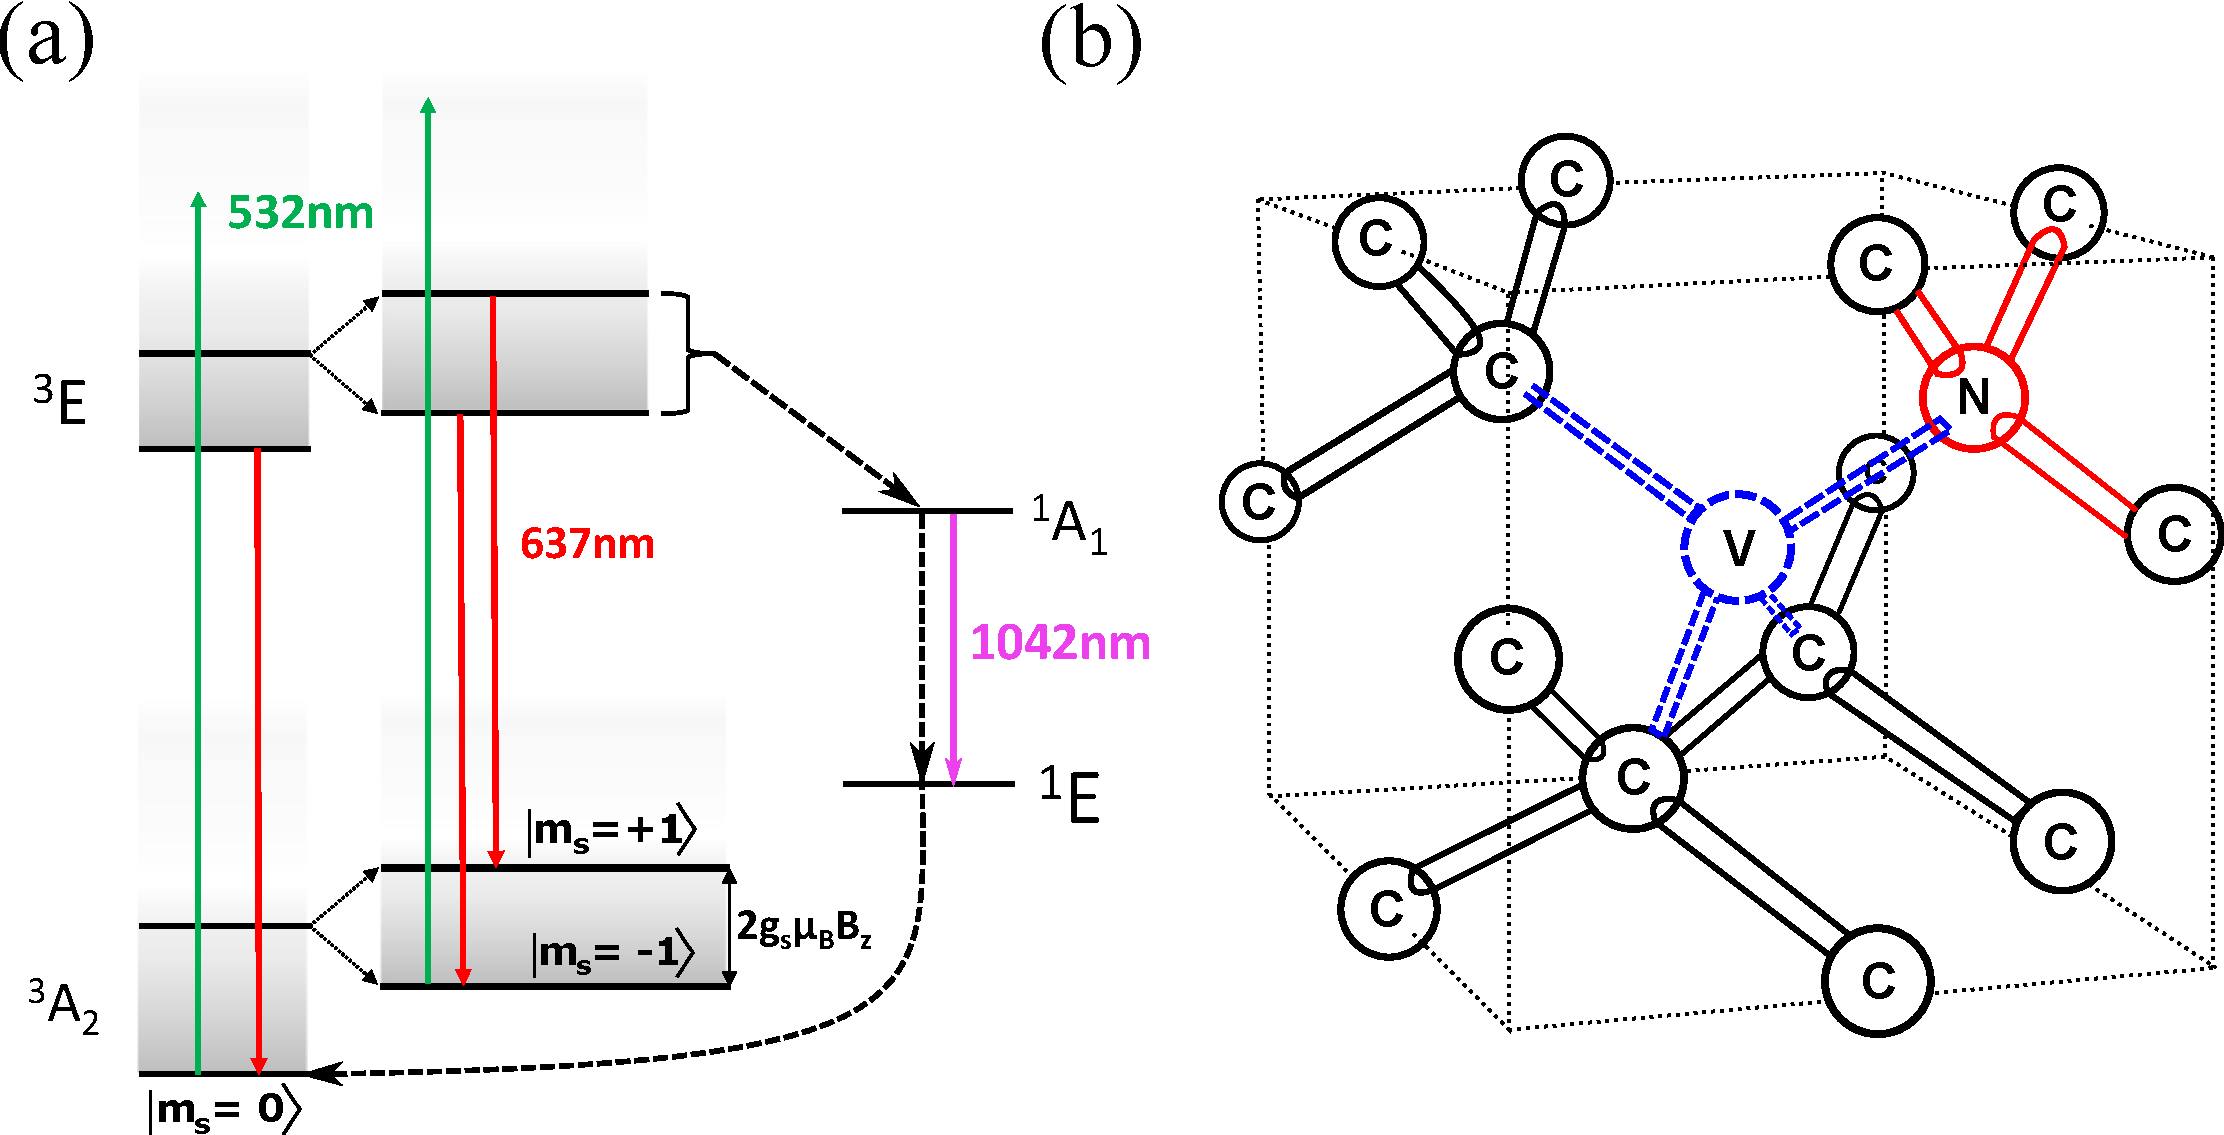
\includegraphics[width =\textwidth]{Intro_Fig_1.pdf}  
\caption{\textbf{The NV center} \textbf{a)} The NV level structure \textbf{b)} One of four crystal orientations of the NV.}
\label{Fig_one}
\end{figure}

\section{Vector Magnetometry with NV Centers}\label{ch1:vect}

As mentioned in section \ref{sec:NVP}, the $C_{3v}$ symmetry of diamond allows NV centers to be aligned in four different orientations in the lattice. Since, at fields lower than 10 mT, the Zeeman splitting of the $\ket{\pm 1}$ is proportional to the vector field projection along the NV symmetry axis\footnote{At these low fields the terms in the NV Hamiltonian (see equation \ref{equ:NVHam}) that are proportional to the perpendicular component of the field are suppressed to order $\sim B_{xy}^2 / D_{gs}$ and can therefore be neglected\cite{taylor2008high}} ($B_z$) the energy shifts can be determined by $\text{g}_\text{s} \upmu \text{b}\textbf{B} \cdot \textbf{\text{u}}_n$ where $\textbf{\text{u}}_n$ ($n = 1,2,3,4$) is the unit vector along the n\textsuperscript{th} NV axis. By either sequentially or simultaneously measuring the Zeeman splitting between either the $\ket{0} \leftrightarrow \ket{+1}$ or $\ket{0} \leftrightarrow \ket{-1}$\footnote{The transition $\ket{-1} \leftrightarrow \ket{+1}$ can also be employed which yields the benefit that the energy shift becomes $2\text{g}_\text{s}\upmu_\text{b}\textbf{B}$ and therefore provides twice the signal over the other two transitions while simultaneously mitigating temperature effects \cite{neumann2013high}. However, this requires treatment of the full three-level spin system since the $\ket{-1} \leftrightarrow \ket{+1}$ splitting is a non-dipole allowed transition.} transitions of all four orientations, one can reconstruct the total vector field by generating the vector components ($B_x$, $B_y$, and $B_z$) from the projection along each of the crystallographic axes \cite{kitazawa2017vector,schloss2018simultaneous}.

\subsection{NV Ensemble Magnetic Sensitivity}



%Talk about spin projection noise, photon shot noise, minimum detectable field \delta B, SNR etc.... see Scott and Chris's thesis

%need to mention \beta, collection rate, C contrast etc here because I use it in the sections below ----- and ODMR

%Talk about using N NVs to enhance sensitivity (look up Hannah paper how they calculate)

% Talk about how sensitivity in an ensemble is increased by 1/sqrt{N} but denser packing of N reduces T_2^* and therefore broadens the minimum achievable bandwidth in an NV experiment.

% Optional: Briefly talk about other readout mechanisms like photoelectric readout, IR absorption readout etc.

\subsection{Continuous Wave Magnetometry}

For continuous wave magnetometry the ESR frequencies are continuously monitored (often using lock in amplification) since the external magnetic field is imprinted in their spectral positions $\omega_+$ and $\omega_-$ [Fig \ref{fig}]. As mentioned in section \ref{ch1:vect}, the four orientations of the NV in the diamond crystal lattice therefore result in eight distinct resonances when split by an external biasing field ($B_0$). Monitoring a minimum of three out of four resonances allows for the full vector reconstruction of the field. An infinitesimal additional magnetic field variation $\delta B$ shifts the resonances away from the known spectrum and the change in NV fluorescence, which is given by $\left(\frac{\partial \beta}{\partial B}\right) \cdot \delta B \cdot \tau$ \cite{rondin2014magnetometry}, is measured in the laboratory. The shot-noise limited sensitivity is then given as,

$$ \eta_{cw} \approx \frac{\hbar}{\text{g}_\text{s} \upmu_\text{B}} \frac{\Delta \omega \sqrt{\tau}}{C\sqrt{N \beta}}. $$  

The signal contrast $C$ can be increased by driving the NV with stronger MW fields at the expense of power-broadening the linewidth $\Delta \omega$. However, the linewidth can be decreased down to a limit given the inhomogeneous dephasing time $T_2^*$ by reducing the laser and MW excitation strength \cite{dreau2011avoiding}, effectively decreasing the number of collected photons per measurement $\beta$. An optimization of contrast $C$, linewidth $\Delta \omega$, and collection $\beta$ yields an optimized sensitivity of \cite{pham2013magnetic}

$$ \eta_{cw} \approx  \frac{2\hbar}{\text{g}_\text{s} \upmu_\text{B}} \frac{1}{C\sqrt{N \beta T_2^*}} . $$

\subsection{Pulsed Ramsey-type Magnetometry} \label{Pulsed_Ramsey}

Strong microwave driving in a CW experiment broadens the ESR linewidth causing a reduction in magnetometer sensitivity. To take advantage of strong driving fields without incurring the effects of MW or pump laser power broadening, DC fields can be measured using a Ramsey pulse sequence. In this scheme microwave driving, spin polarization and sensing are all separated in time [Fig \ref{Fig_two}(a)]. After spin polarizing the NV electron spin into the $m_s = 0$ ground state, a resonant microwave pulse of length $\pi/2$ creates a superposition of the $\ket{0}$ and $\ket{+1}$ energy levels,
$$\ket{\Psi} = \frac{1}{\sqrt{2}}(\ket{0} + e^{i\phi}\ket{1}),$$
where the accumulated phase after precession time $\tau$ is $\phi = 2\pi \gamma B \tau$ where $B$ is the amplitude of the magnetic field to be determined and $\gamma = \text{g}_\text{s} \upmu_\text{B} / h = 2.8$ MHz/gauss the NV electron spin gyromagnetic ratio. Following the precession interval, a second $\pi/2$ MW pulse projects the spin back onto the quantization axis which is measured in the laboratory as a population difference between $\ket{0}$ and $\ket{+1}$, and read out optically through the spin dependent fluorescence of the NV center. Sensitivity is therefore improved by increasing the free precession time $\tau$ in order to maximize the accumulated phase, however, dipolar coupling to other magnetic impurities in the spin bath randomizes the accumulated phase after time $T_2^*$, the inhomogeneous NV dephasing time. Sensitivity in this scheme is optimized when the NV is allowed to precess in the magnetic field for $\tau \sim T_2^*$ and is given by 

$$\eta_{ramsey} \sim \frac{\hbar}{\text{g}_\text{s} \upmu_{\text{B}}} \frac{1}{C\sqrt{N \beta T_2^*}}.$$ 

\begin{figure}[t!]
\centering
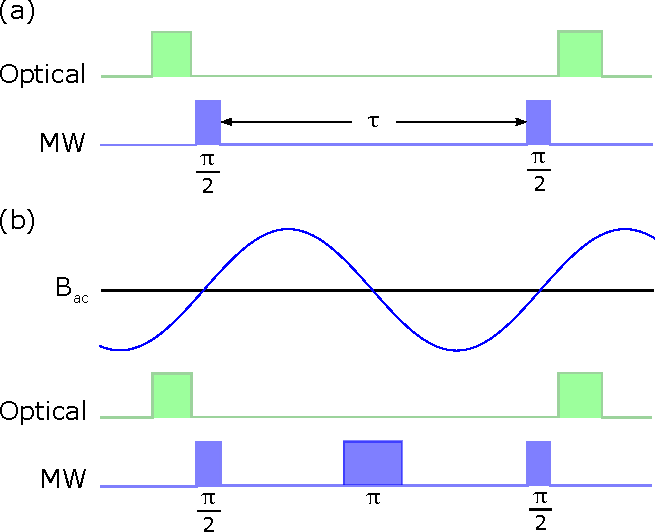
\includegraphics[scale = 0.9]{Ramsey_DC_AC.pdf}  
\caption{\textbf{Pulsed Magnetometry Sequences} \textbf{a)} Ramsey Sequence for DC magnetometry \textbf{b)} Hahn-Echo Sequence for AC magnetometry.}
\label{Fig_two}
\end{figure}

For AC magnetometry, the Ramsey sequence can be modified by bisecting the free precession interval $\tau$ with a single resonant $\pi$ pulse. The pulse is precisely timed to occur at the node of the oscillating field [Fig \ref{Fig_two}(b)] and deems to swap the accumulated phase from the $\ket{1}$ to the $\ket{0}$ state. For slow components of the external magnetic noise, the swap allows the second half of the free precession interval to compensate for phase randomization acquired during the first half of the interval. Using this sequence, $\tau$ can be increased to the homogeneous spin coherence time $T_2$ often orders of magnitude longer than $T_2^*$. The sensitivity for sensing an AC field is then improved when compared to sensing a DC field by a factor $\sqrt{T_2^*/T_2}$. This sequence is known as a Hahn-Echo sequence but AC magnetometry can be performed by more complex dynamical decoupling techniques \cite{carr1954effects, meiboom1958modified}.


\subsection{Rabi oscillations}

When an on- or near-resonant MW pulse is applied to a ground state transition in the NV, e.g. $\ket{0} \rightarrow \ket{+1}$, the NV spin state population will oscillate coherently between these two levels at a rate called the Rabi frequency ($\Omega_R$). This rate of oscillation is a function of the amplitude of the applied MW pulse. It is commonly measured by consecutively applying a polarizing laser pulse, a MW pulse, and a readout pulse [Fig. \ref{Fig1_3} (a)] and varying the MW pulse length after each iteration. 

\begin{figure}[t!]
\centering
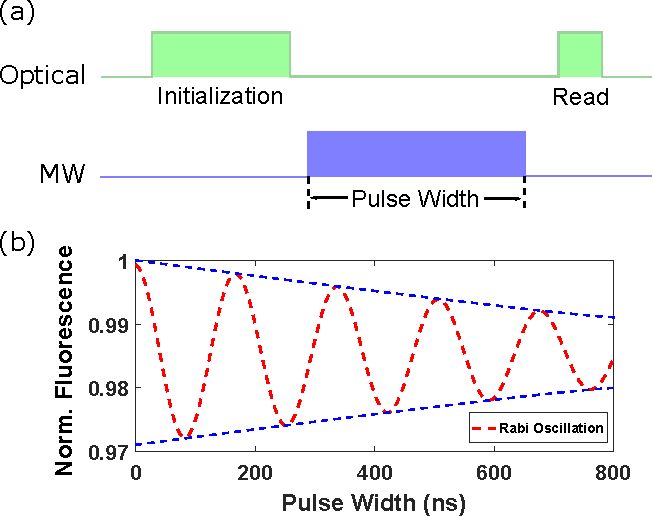
\includegraphics[scale = 0.9]{Rabi_sequence_and_figure.pdf}  
\caption{\textbf{Rabi pulse sequence and oscillations} \textbf{a)} Pulse sequence for detecting Rabi oscillation between two spin sublevels \textbf{b)} Example Rabi oscillations (\textcolor{red}{-- --}) with exponential decay envelope (\textcolor{blue}{ -- --}).}
\label{Fig1_3}
\end{figure}

Fig. \ref{Fig1_3} (b) plots a typical Rabi curve and its decay envelope. If the NV is originally in $\ket{0}$ (ie. at time $t = 0$) and we let the system evolve, then the probability that the spin is found in $\ket{+1}$ is $P_{+1} = \left(\frac{\omega_1}{\Omega_R}\right)^2 sin^2\left(\frac{\Omega_R t}{2}\right)$ where $\Omega_R = \sqrt{(\omega-\omega_0)^2-\omega_1^2}$ is the Rabi frequency, $\omega$ is the radial frequency of the oscillating field $B_1(\omega)$, $\omega_0$ the resonant frequency of the transition, and $\omega_1$ the (max) Rabi frequency at zero detuning. At resonance, the driving frequency is $\omega = \omega_0$ and the transition probability becomes $P_{+1} = sin^2\left(\frac{\omega_1 t}{2}\right)$. In order to therefore drive the entire population from e. g. $\ket{0}$ to $\ket{+1}$ as needed in, for example, the Hahn-Echo sequence described in \ref{Pulsed_Ramsey}, one needs to apply a pulse length such that $sin^2 \left(\frac{\omega_1 t}{2}\right) = 1$ which is satisfied when $t = \frac{pi}{\omega_1}$. For a Ramsey-type sequence that requires an equal superposition between $\ket{0}$ and $\ket{+1}$ one needs to apply half the $\pi$ pulse, $t = \frac{\pi}{2\omega_1}$. The Rabi oscillations however decay due to inhomogeneous broadening of the ensembles linewidth, and are therefore fit by the decaying envelope $\text{exp}\{-\left(PW/T\right)^p\}$, where PW is the pulse width and $T$ and $p$ are fit parameters.

\section{NV-MW coupling}

calculate coupling between NV center and MW photons in cavity.

%% This is an example first chapter.  You should put chapter/appendix that you
%% write into a separate file, and add a line \include{yourfilename} to
%% main.tex, where `yourfilename.tex' is the name of the chapter/appendix file.
%% You can process specific files by typing their names in at the 
%% \files=
%% prompt when you run the file main.tex through LaTeX.

\chapter{The Loop Gap Resonator}

As mentioned in the introduction, for many applied modalities within applications that use NV centers, the MW field (often denoted $B_1$ from NMR nomenclature), requires both high power and high uniformity to achieve high-fidelity quantum-state manipulation over the entire sample volume. As volumes are increased however, to maximize the number of NVs addressed without having a deleterious affect on the optimal measurement time, applying such a field becomes more difficult using standard approaches such as shorted coaxial loops \cite{clevenson2015broadband,chipaux2015magnetic}, microstrip waveguides \cite{andrich2017long,horowitz2012electron}, and 50 $\Omega$-terminated coaxial transmission lines \cite{li2010design,mrozek2015circularly,zhang2016microwave,zhang2018vector}. These broadband approaches allow arbitrary drive frequencies, however, the lack of resonant enhancement forces a compromise between the addressed volume and field strength. Section \ref{Planar} describes how planar lumped-element resonators such as split-ring resonators \cite{bayat2014efficient}, planar-ring resonators \cite{zhang2016microwave,sasaki2016broadband}, omega resonators \cite{twig2013ultra,horsley2018microwave,simpson2017electron}, and patch antennas \cite{zhang2016microwave} can improve coupling between the resonator and the NVs by resonantly enhancing the local $B_1$ field and thus enable MW driving over larger regions, but at the expense of bandwidth and thus, for an operational magnetometer, dynamic range. Additionally, planar resonators are shown to yield poor homogeneity in the planes normal to their surface and therefore lend themselves less to bulk magnetometry than to 2D imaging applications. To address this shortcoming 3D resonators and cavities can be employed such as enclosed metallic cavity resonators \cite{rose2017coherent}, enclosed dielectric resonators \cite{breeze2017continuous,floch2016towards,creedon2015strong}, open dielectric resonators \cite{kapitanova2017dielectric}, and three-dimensional lumped element resonators \cite{angerer2016collective}, which provide good field homogeneity and strong resonantly enhanced fields, but offer little to no optical access. Since all-optical initialization and readout is a primary benefit for many solid-state spin systems, including NV diamond \cite{doherty2013nitrogen}, such a trade-off is incompatible with many existing and envisioned applications \cite{schirhagl2014nitrogen}. 

To address this current shortcoming a three-dimensional tunable loop-gap resonator (LGR), based on the anode block of a cavity magnetron, is used to achieve desired MW drive strengths homogeneously over large areas. Additionally, its open geometry allows for good optical accessibility for interrogation volumes centered within the LGR cavity. Traditionally, the LGR has been used either as the anode block of cavity magnetrons \cite{}, or as a low frequency (2-4 GHz) lumped element resonator for electron paramagnetic resonance (EPR) studies \cite{}.  

\section{Resonant Enhancement of the MW field}\label{resonant_enhc}

The LGR acts classically like an underdamped oscillator. It stores MWs within the confines of its geometrical structure by allowing the energy to oscillate back and forth between an electric and magnetic potential. At resonance ($\omega_0$) the ratio of magnetic energy to electric energy is 1. The time $\tau_{ring}$ the energy can oscillate before its power is reduced by a factor of 1/e is characterized by a dimensionless quantity called the Q-factor. It's defined by the following ratio
\begin{equation}
Q = \omega_0 \frac{Stored Energy}{Power Loss}.
\end{equation}
If the resonator is therefore continuously fed by an external power source an enhancement of the stored energy takes place that is proportional to the Q-factor of the cavity. The magnitude of the magnetic flux within the center cavity (for a cylindrical resonator) is given by
\begin{equation}
|B_1| \approx  2\left[\frac{\upmu_0}{\omega V_r}\right]^{1/2} \cdot \sqrt{P_0} \cdot \sqrt{Q},
\end{equation}
where $\upmu_0$ is the vacuum permeability, $P_0$ is the power coupled to the resonator, $\omega$ is the angular frequency, and $V_r$ is the volume of the center loop. It's therefore clear that a resonant enhancement of the magnetic field amplitude is induced which is proportional to the square root of the Q-factor. 


\section{Model}

The following sections build a model of the LGR both as an equivalent circuit and as solutions to Maxwell's equations for the LGR's geometry. Figure \ref{LGR_geometry1} shows the LGR with geometrical parameters used in the following sections. The focus here lies on hole-and-slot type LGR resonators since this variation is designed and used in the rest of this thesis. Other types of resonators are shown in section \ref{LGRDesignSection} Figure \ref{LGR_variation}.


\begin{figure}[h!]
\centering
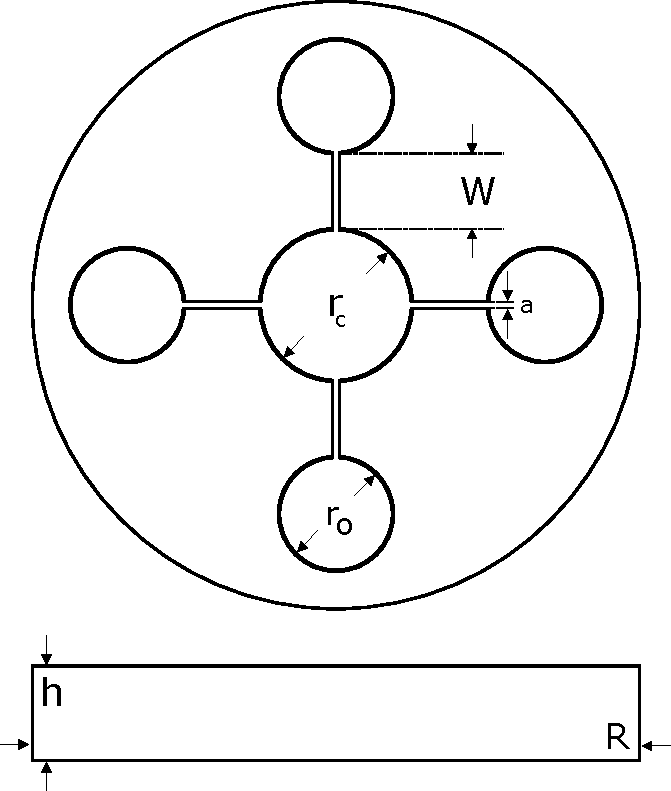
\includegraphics[scale = 0.55]{LGR_geometricalParams.pdf}  
\caption{\textbf{LGR dimensions} Geometrical parameters of LGR used in sections \ref{circuit}, \ref{fields} and \ref{coupling}}
\label{LGR_geometry1}
\end{figure}


\subsection{Resonant frequency using equivalent circuit} \label{circuit}

\begin{figure}[t!]
\centering
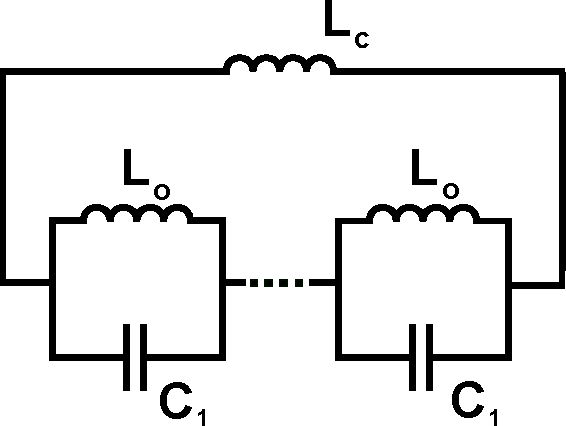
\includegraphics[scale = 0.9]{circuit_drawing.pdf}  
\caption{\textbf{LGR equivalent circuit diagram} Diagram showing equivalent inductance and capacitance of LGR and their connections.}
\label{circuitdiagram}
\end{figure}

The LGR can be modeled by an equivalent circuit in which the gaps behave like capacitors and the loops like inductors. It's important to note that such a picture neglects effects such as radiation losses or fringing fields that extend into space above and below the LGR. However these effects can be incorporated with considerable effort and are described in detail within the following references \cite{mehdizadeh1983Loop, rinard2005loopgap, wood1984loop}. For an $m$ loop and $n$ gapped LGR, the equivalent circuit is depicted in Figure \ref{circuitdiagram}. Using the variables given in Figure \ref{LGR_geometry1}, the charge at the gap walls creates a capacitance $C_1$, and circulating currents around each loop create an inductance $L_1$
\begin{equation} \label{indcap}
C_1 \approx \frac{\epsilon_r \epsilon_0 W h}{a}, \quad L_1 \approx \frac{\mu_0 \pi r_i^2}{h}, 
\end{equation}
where $r_i$ is the radius of either loop ($i \equiv o,c$). Using circuit analysis we can solve the diagram in Figure \ref{circuitdiagram} for the total capacitance, $C$,
\begin{equation}\label{capacitance}
C = \frac{C_1}{n},
\end{equation} 
and total inductance, $L$,
\begin{equation}\label{inductance}
L = \frac{n L_o L_i}{n L_o + L_i}.
\end{equation}
The resonant frequency of the LGR is therefore given by 
\begin{equation}
f_0 = \frac{1}{2 \pi \sqrt{LC}}
\end{equation}


\subsection{Solution to Maxwell's equations} \label{fields}

The full derivation of the solutions to Maxwell's equations for an $n$ gap LGR can be found in reference \cite{piasecki1993field}. However, this chapter is intended to give a brief overview of the solutions. In general, Maxwell's equations for the LGR center cavity can be solved by using Bessel and Neumann functions which are generally found to be the solutions to finite length cylindrical waveguides \cite{}. Neumann functions however are singular at the origin and therefore only Bessel functions (of the first kind) need to be considered. The full solution then takes the form
\begin{equation}
H_z^{(p)} = \mathcal{J}_p(k\rho) e^{i p \phi}.
\end{equation}
Where we are operating in cylindrical coordinates and $\mathcal{J}_p$ is the $p^{th}$ order Bessel function and $k = \omega \sqrt{\mu_0\epsilon_0}$. If we assume that the field in the center is fully directed in $z$ then the boundary condition for the magnetic field becomes
\begin{equation}
H_z = H_z(\rho,\phi)e^{i\omega t}, \quad H_{\rho} = H_{\phi} = 0.  
\end{equation} 
Solving Maxwell's equations then yields



\subsection{Coupling} \label{coupling}

Theory of coupling (mutual inductance, capcitance, etc)

\section{LGR Design} \label{LGRDesignSection}

Due to the loop gap resonator's existence since the early 20th century \cite{collins1948microwave} it has seen many variations and modifications all designed with particular applications in mind. Figure \ref{LGR_variation} shows the cross section of a variety of LGRs including rising-sun, vane, slot, and hole-and-slot type resonators. EPR experiments at low frequencies (2-4 GHz) quickly adopted the LGR as opposed to more traditional TE\textsubscript{102} type cavities because of the LGRs smaller size relative to the frequency of excitation. At 3 GHz the side length of the TE\textsubscript{102} cavity must be at least 5 cm which reduces drastically the cavity filling factor--a parameter necessary for the sensitivity of an EPR signal. Since many aspects of EPR spectroscopy are mirrored in NV magnetometry (requirement of homogeneous and strong microwave signals, frequency of operation, etc.) we selected to design a hole-and-slot type resonator found in many EPR applications \cite{}.  
\vspace{5mm}
\begin{figure}[h!]
\centering
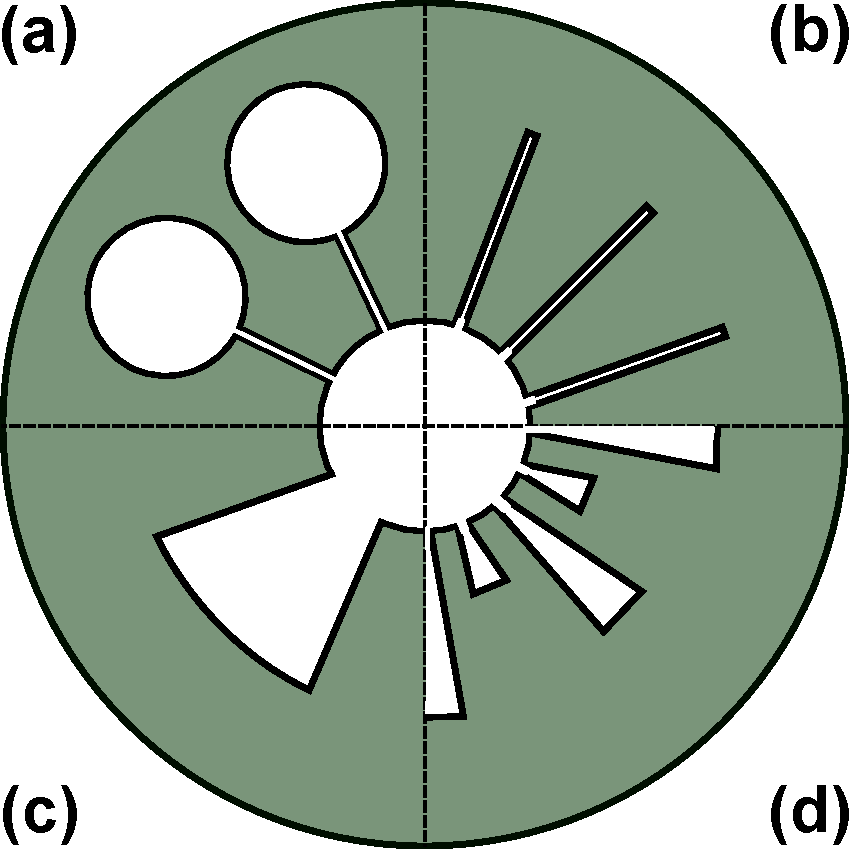
\includegraphics[scale = 0.5]{LGR_Variation.pdf}  
\caption{\textbf{Loop Gap Resonator Variations} \textbf{a)} Hole and Slot. \textbf{b)} Slot. \textbf{c)} Vane. \textbf{d)} Rising Sun - type}
\label{LGR_variation}
\end{figure}


\subsection{LGR}

A standard hole-and-slot LGR with $n$ outer loops can be approximated as $n$ coupled LC resonators oscillating in tandem at a target resonant frequency \cite{wood1984loop}. Circulating currents around the central and outer loops create a total inductance \ref{inductance}, and charge at the gaps creates the total capacitance \ref{capacitance} as found in section \ref{circuit}. In practice, the central loop diameter is set to $\sim 5-10 $ mm, corresponding to the typical size of a diamond plate. The outer loop diameters are chosen to match the inner diameters within a small factor to ensure return flux is captured and does not extend into the annular region around the LGR \cite{}. Since the outer and inner loops set the effective inductance of the resonator, the gap area $A = h \times W$ is constrained by the dual LGR design objectives of (i) maintaining optical accessibility, which limits the thickness of the device, and (ii) bounding $f_0$ above the target resonant frequency in order to allow for further tuning vie dielectric shims (discussed in section \ref{tuning}). Additionally, while increasing the number $n$ of loops and gaps can improve $B_1$ uniformity \cite{piasecki1993field} and lower the LGR's resonant frequency, this approach results in a denser mode spectrum \cite{froncisz1982loop} and increases the likelihood of cross-mode excitations deleteriously altering the field distribution within the central loop. As a compromise, the design employs $n=4$ outer loops [Fig. \ref{LGR_drawing} (a)] allowing for sufficient uniformity while locating the closest eigenmode more than 1.5 GHz below the TE\textsubscript{10} eigenmode [Fig \ref{}].  

\begin{figure}[b!]
\centering
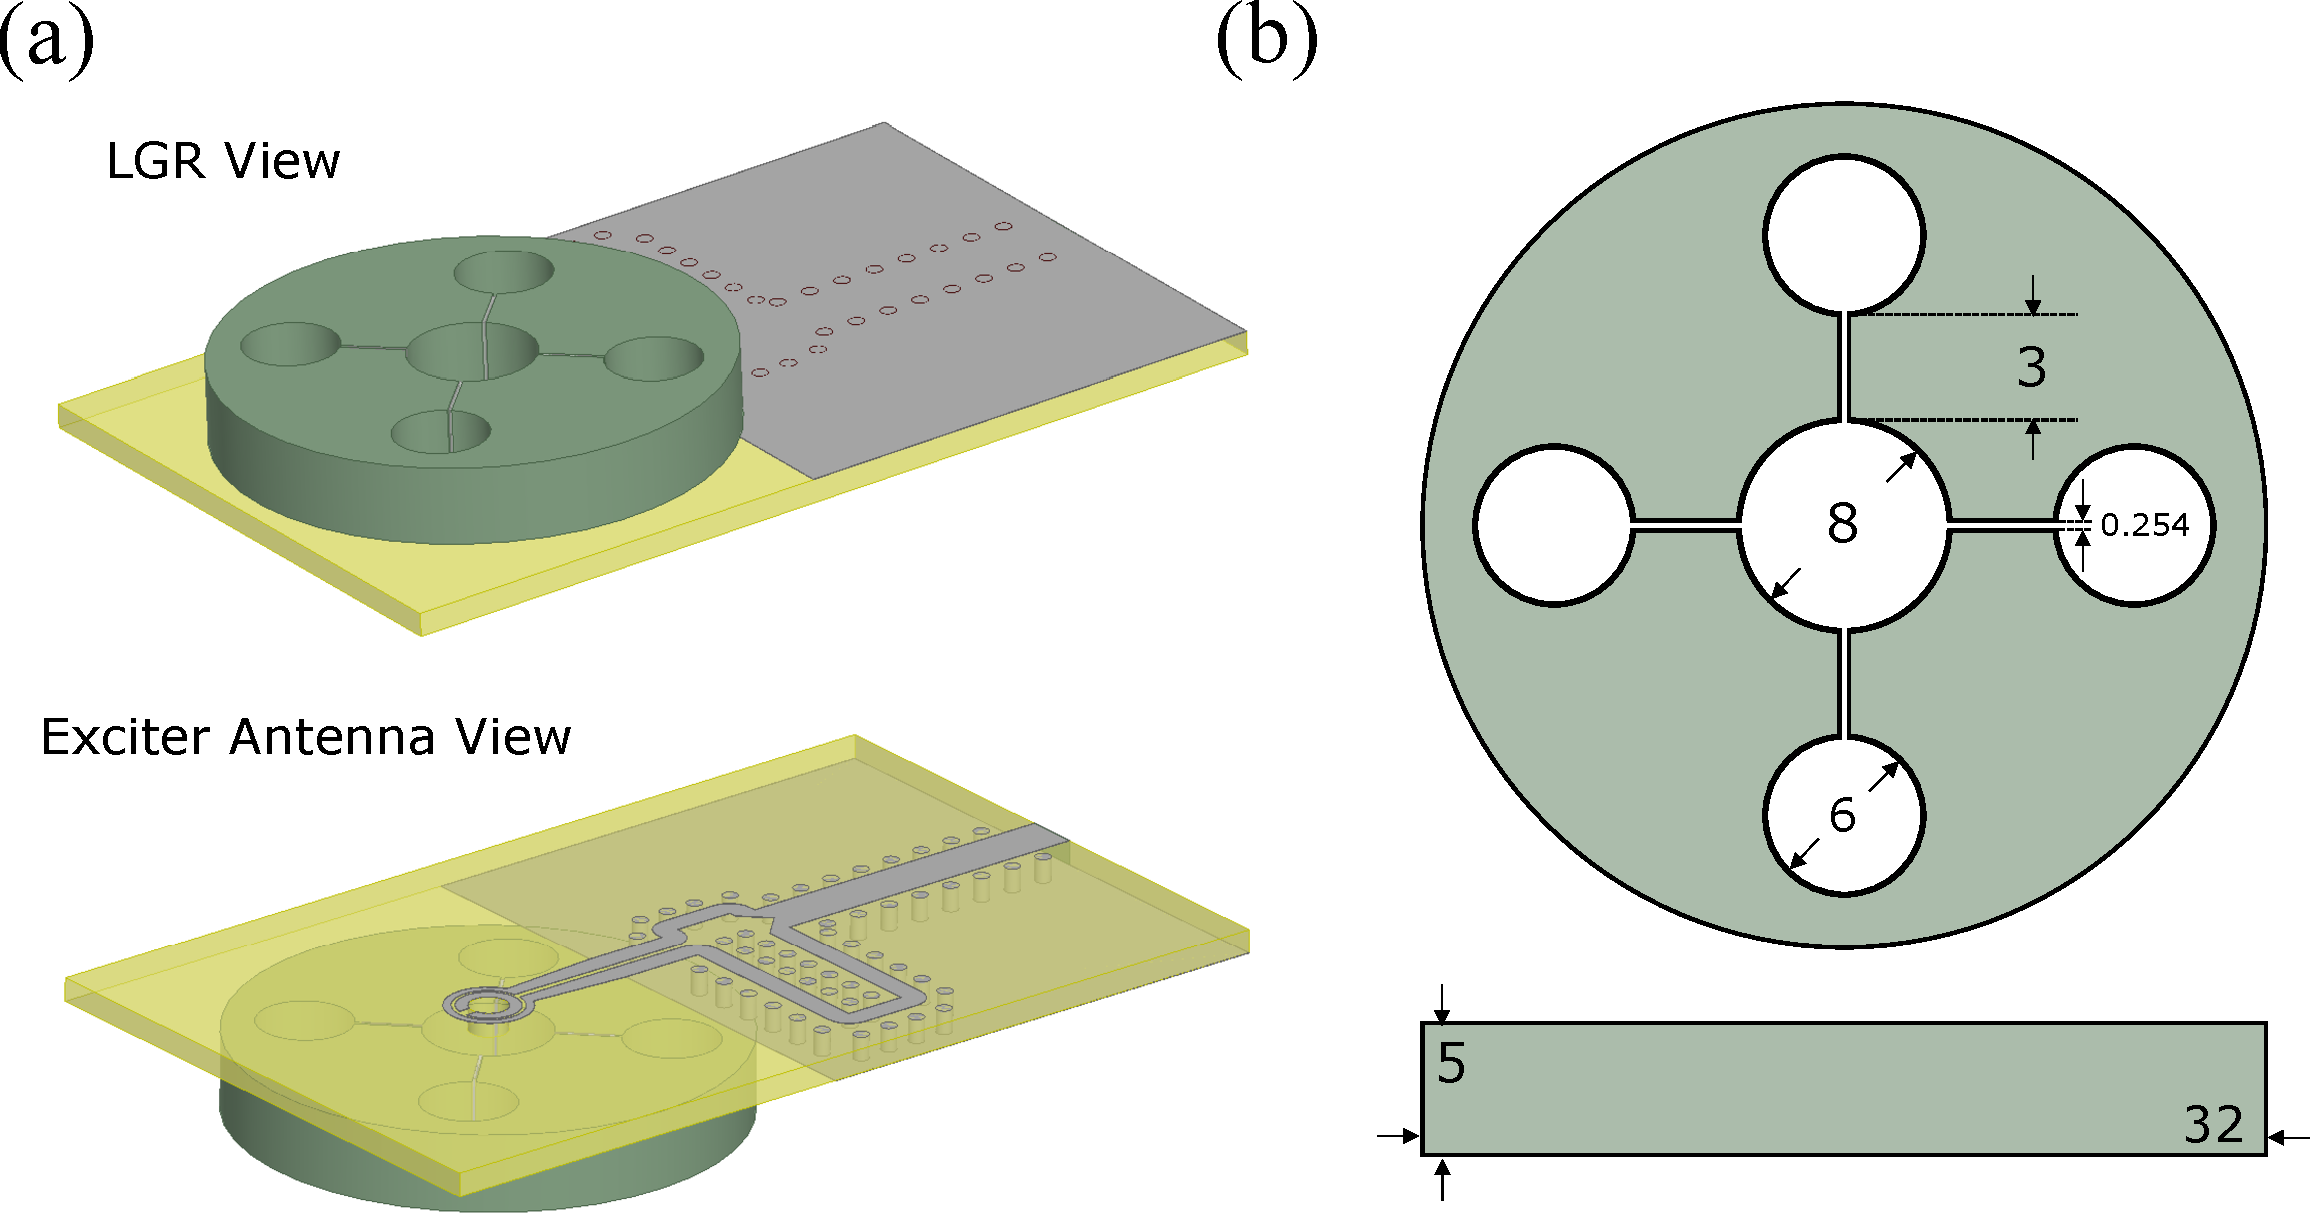
\includegraphics[width = \textwidth]{LGR_Image.pdf}  
\caption{\textbf{Rendering and Wire Diagram of Loop Gap Resonator} \textbf{a)} The metallic resonator employs a five-loop four-gap architecture. Microwaves are coupled into the LGR via the exciter antenna, which is fabricated on a printed circuit board. \textbf{b)} Line drawing of the LGR. All dimensions are in mm. Optional mounting holes and radial access port for laser excitation are now shown.}
\label{LGR_drawing}
\end{figure}

%\begin{tabular}{|c|c|}

%\end{tabular}

The LGR in this work therefore consists of a central loop with radius $r_c = 4$ mm surrounded by four symmetrically arranged outer loops of radius $r_o = 3$ mm as shown in Figure \ref{LGR_drawing} (b). The outer loops return magnetic flux to the central loop and therefore oscillate antisymmetrically with the central loop ($\pi$ out of phase). The side walls of the capacitive gaps are separated by $d = 254$ $\upmu$m. With these dimensions, using equations \ref{indcap}, \ref{inductance}, and \ref{capacitance} yield $L = 8.7$ nH and $C = 0.17$ pF, resulting in an expected resonant frequency for the naked air-gapped LGR of $f_0 = 4.1$ GHz, approximately 1.2 GHz above the NV resonance frequencies. An eigenfrequency simulation of the resonator using the geometrical parameters listed above was completed in ANSYS HFSS and the distribution of the magnetic flux density ($B_1$) for the TE\textsubscript{10} mode is depicted in Figure \ref{LGR_Eigen}. As mentioned above, for this mode the center loop oscillates $\pi$ radians out of phase with the outer loops. For the air-gapped resonator, HFSS returns a real eigenfrequency at 4.57 GHz (depicted in Figure \ref{LGR_Eigen}) 

The LGR is fabricated via wire electron discharge machining, which is well-suited for producing the tight tolerances and vertical side walls required for the narrow $d = 254 \upmu$m capacitive gaps. A titanium alloy (Ti-6Al-4V) was chosen as the resonator cavity material. The lower conductivity of this alloy compared to that of copper ($\sigma_{Ti} = 5.8 \times 10^{5}$ S/m vs. $\sigma_c = 59 \times 10^6$ S/m) allows for a broader resonance with a 3dB bandwidth $\Delta_{3dB} = 80$ MHz, sufficient to address all eight NV resonances for bias magnetic fields $B_0$ up to $\sim 20$ gauss. This 80 MHz bandwidth corresponds to a loaded quality factor $Q_L \equiv f_0/\Delta_{3dB} \approx 36$ when the LGR
is critically coupled to the driving source (see section \ref{quality}). The LGR may be optionally fit with a radial access hole (for laser excitation of the NV ensemble) and three \# 2-56 mounting holes, which affix the LGR to an exciter antenna, discussed next.

\begin{figure}[h!]
\centering
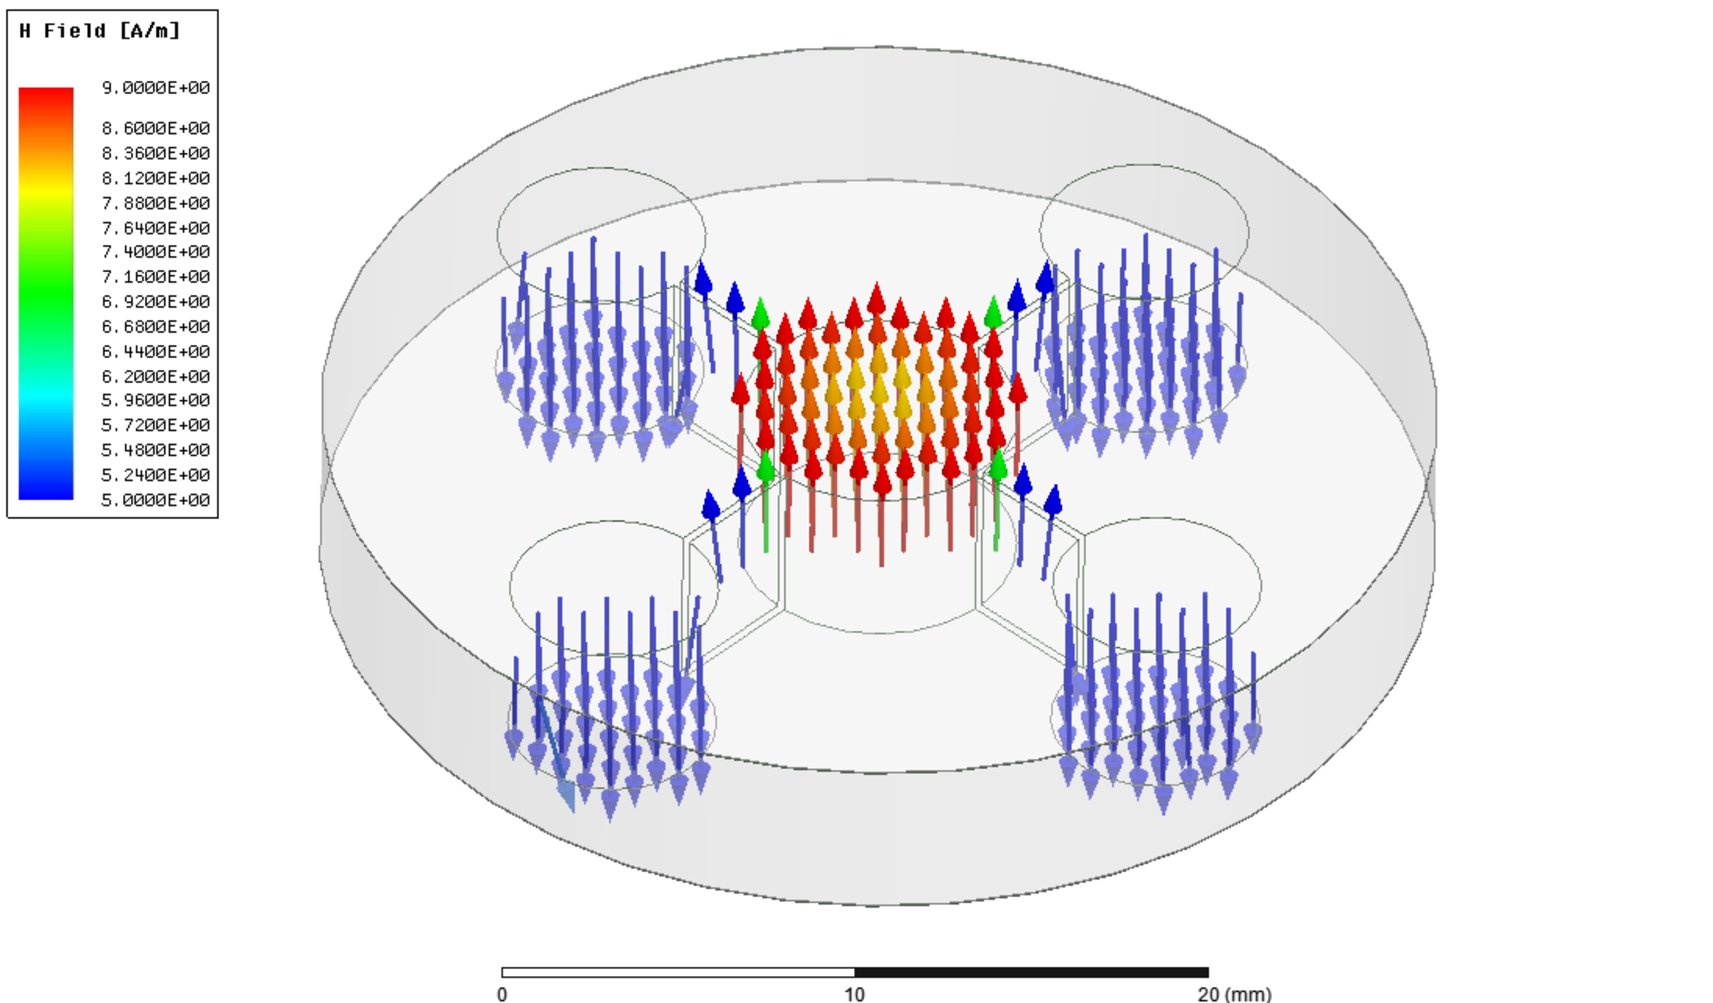
\includegraphics[scale = 0.5]{Eigen_Res.pdf}  
\caption{\textbf{Eigenfrequency solution to LGR} TE\textsubscript{10} mode located at $f_0 \approx 4.6$ GHz. The outer loops are oscillating $pi$ radians out of phase with center loop.}
\label{LGR_Eigen}
\end{figure}


\subsection{Tuning} \label{tuning}

The LGR resonant frequency $f_0$ is additionally tuned by inserting
and translating dielectric shims in the LGR's capacitive
gaps, thereby increasing total capacitance C until $f_0$ overlaps the NV resonance frequencies as desired. Shimming material should be chosen to provide a high dielectric (and thus large tuning range) and low loss tangent (tan $\delta$, where $\delta$ is the inverse skin-depth). We employ 200 $\upmu$m thick C-plane sapphire, which is commercially
available in semiconductor grade 50.8 mm diameter wafers, can be cut on standard wafer dicing saws, has a high relative permittivity of $\epsilon_r = 11$ parallel to the C-plane \cite{westphal1972dielectric}, and exhibits a low dielectric loss of tan $\delta$ < 0.0001 at 3 GHz \cite{westphal1972dielectric, hartnett2006sapphireshim}. The sapphire shims are cut to lengths longer than the $l_c = 4$ mm radial length of the capacitive gaps, wedged into the gaps, and held in place with PTFE thread tape. These sapphire shims are then translated radially until the desired value of $f_0$ is attained. The shims are always positioned so that excess shim length extends into the outer rather than the central loop, in order to minimally perturb the central loop $B_1$ field. Simulations further suggest that radially symmetric shim configurations produce the best $B_1$ field homegoneity, as asymmetries in shim placement perturb the desired TE\textsubscript{01} field distribution. 



\subsection{Excitation Design}

To couple MW power into the LGR we utilized two separate methods, each to be used for different NV applications. For magnetic  microscopy, complete 2$\pi$ steradian optical access to the center cavity is of the utmost importance. For such modalities lateral coupling using a shorted coaxial loop [Figure \ref{LGR_Lateral} (a)] can be used to minimize the blocking of optical access to the central loop \cite{koskinen1992the}. Using this method, resonator coupling (described in section \ref{coupling}) is modified by changing the coaxial loop position in $z$ relative to the LGR. In this way the LGR can be quickly and effectively critically coupled for any shim configuration (ie. resonant frequency) [Figure \ref{LGR_Lateral} (b)]. Note that changing the coupling loop distance affects the mutual inductance between the shorted-loop and the resonator. As an undesired consequence, the resonant frequency of the total device shifts away from the frequency it was initially tuned to. A simple optimization process however, that can often be accomplished by hand, between shim placement and loop-LGR distance can lead to the desired coupling at the targeted frequency.

\begin{figure}[t!]
\centering
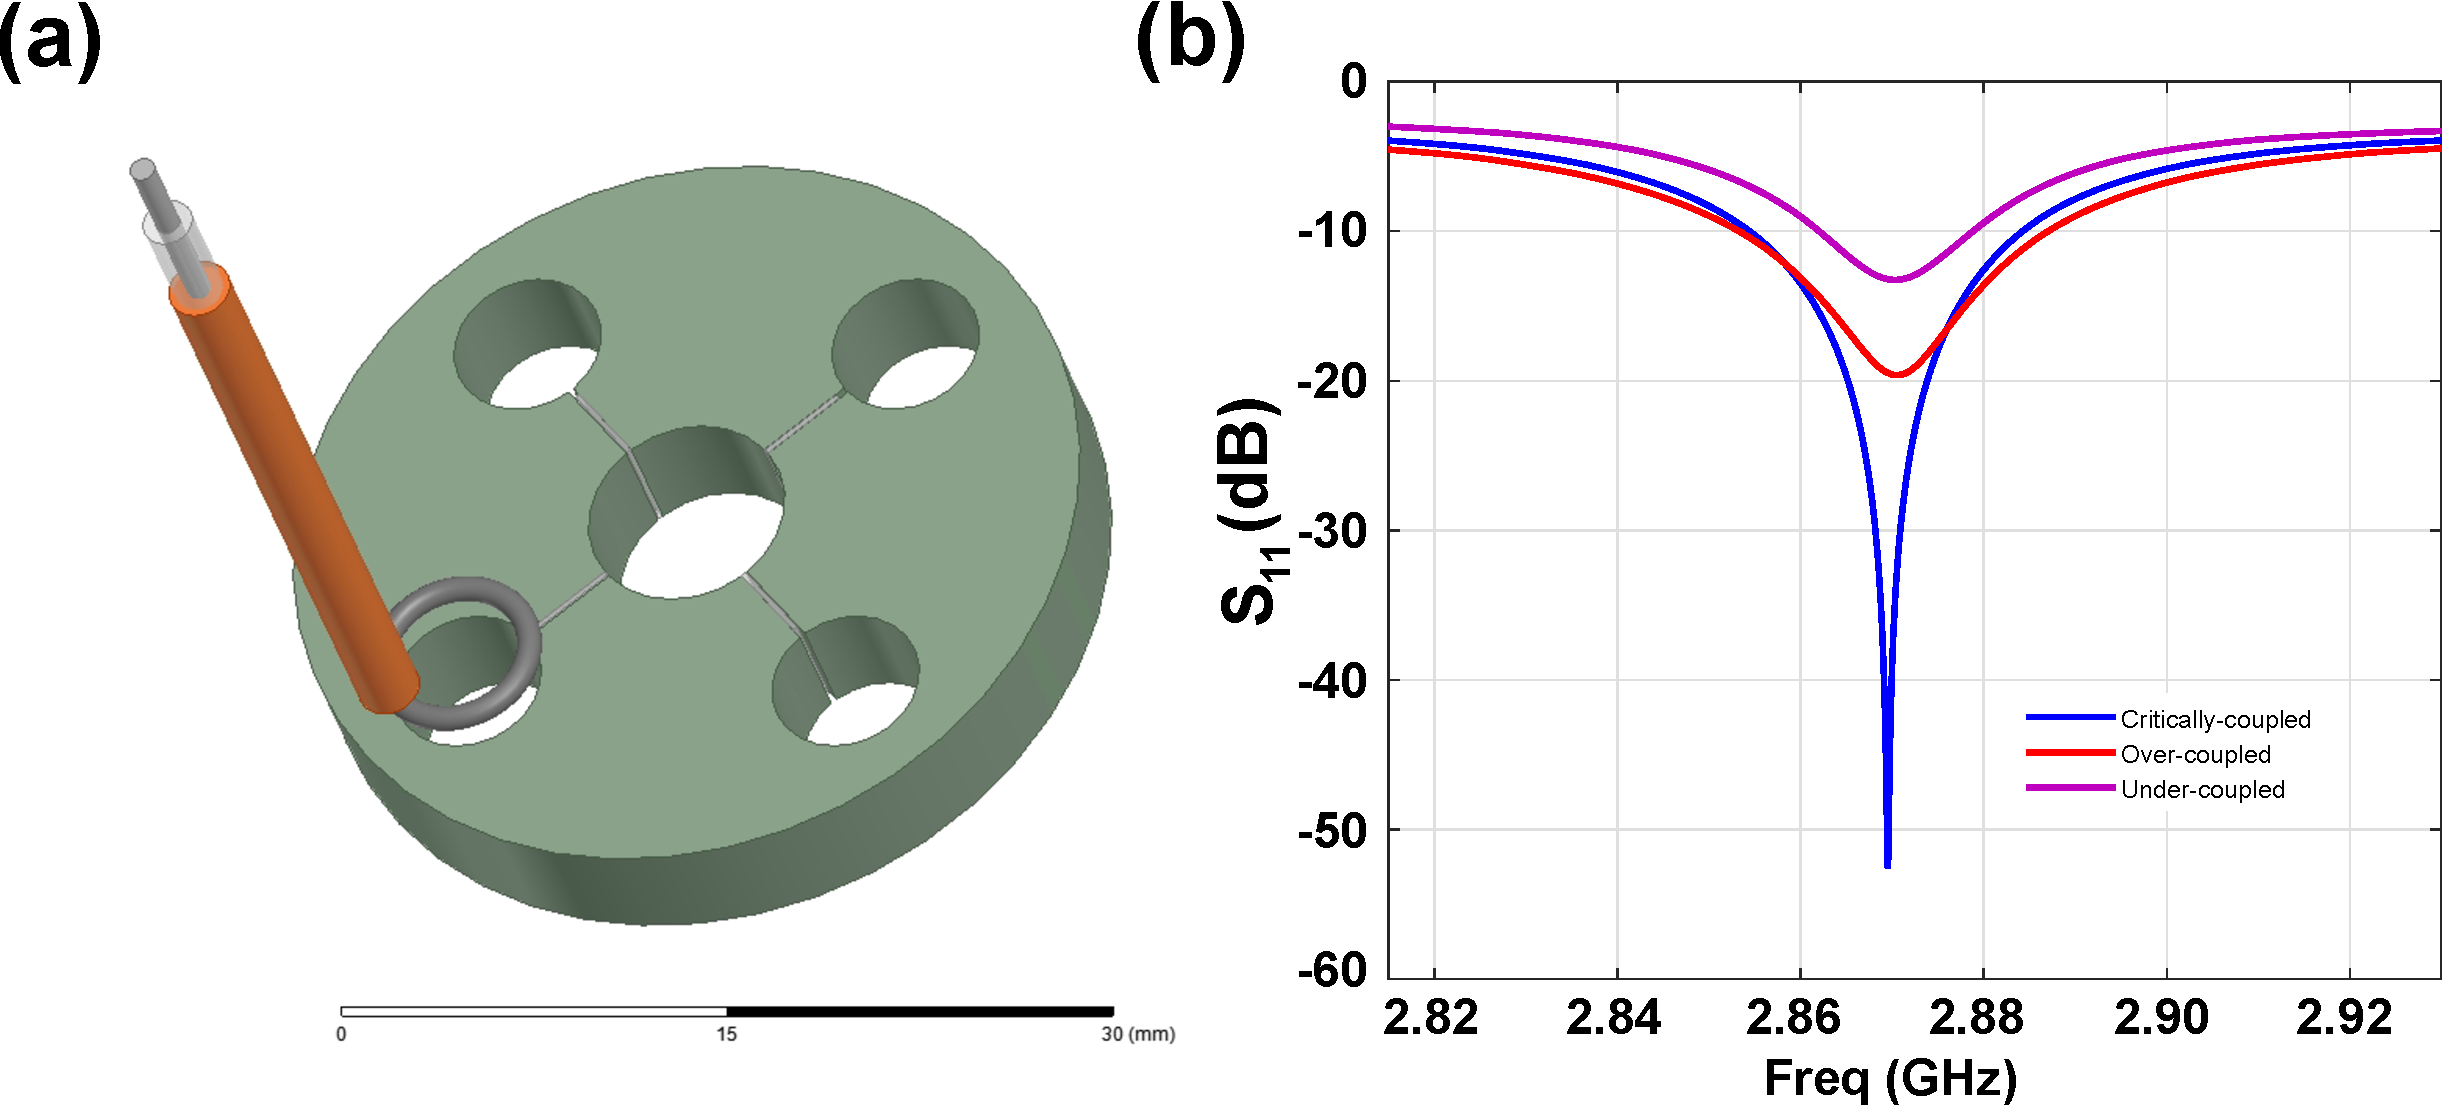
\includegraphics[width = \textwidth]{Lateral_Coupling.pdf}  
\caption{\textbf{3D Rendering of coupling loop and scattering parameter for different coupling configurations} \textbf{a)} Rendering of lateral coupling loop and LGR. \textbf{b)} Scattering parameter $S_{11}$ for different coupling configurations. Critically coupled (\textcolor{blue}{\textbf{---}}) at $z \approx 1$ mm, under-coupled (\textcolor{red}{---}) at $z \approx 1.25$ mm, over-coupled (\textcolor{purple}{---}). }
\label{LGR_Lateral}
\end{figure}

The purpose of the second devised coupling method is to provide a mechanically stable and wide bandwidth match for a future field-able NV magnetometer. While the lateral-loop coupling approach yields near perfect optical access to a sample placed in the center loop of the LGR, the long lever arm of the coaxial cable is susceptible to pertubation in a non-laboratory setting. An oscillation in the coupling loop manifests itself in an oscillation in the value of the coupling parameter $\beta$ and, in effect, an oscillation of the LGR resonant frequency and MWs supplied to the NVs. For applications that can sacrifice optical access, such as a bulk field-able magnetometer, we design a split-ring coupling structure on a dielectric substrate which is subsequently mounted on the LGR [Figure \ref{LGR_drawing} (a)]. The fixed distance between the split-ring and LGR prevents quick "on-the-fly" coupling when the device is shim-tuned to another resonant frequency. Therefore the device must be well coupled across a wide bandwidth, which can be achieved using a balun (\textbf{ba}lanced-\textbf{un}balanced) placed between the feed-line and the exciter antenna (split-ring resonator). Figure \ref{LGR_Exciter} shows the exciter board composed of a 50:50 power splitter, a balun and a split-ring resonator. The balun is designed to match the exciter antenna to the LGR over a minimum bandwidth of 1 GHz centered at the zero-field splitting of the NV (D\textsubscript{gs}). The 2D electromagnetic simulation tool Sonnet was used to ensure a flat $S_{21}$ and $S_{31}$ response between the feed-line and split-ring exciter antenna over the frequency range in question. 

\begin{figure}[t!]
\centering
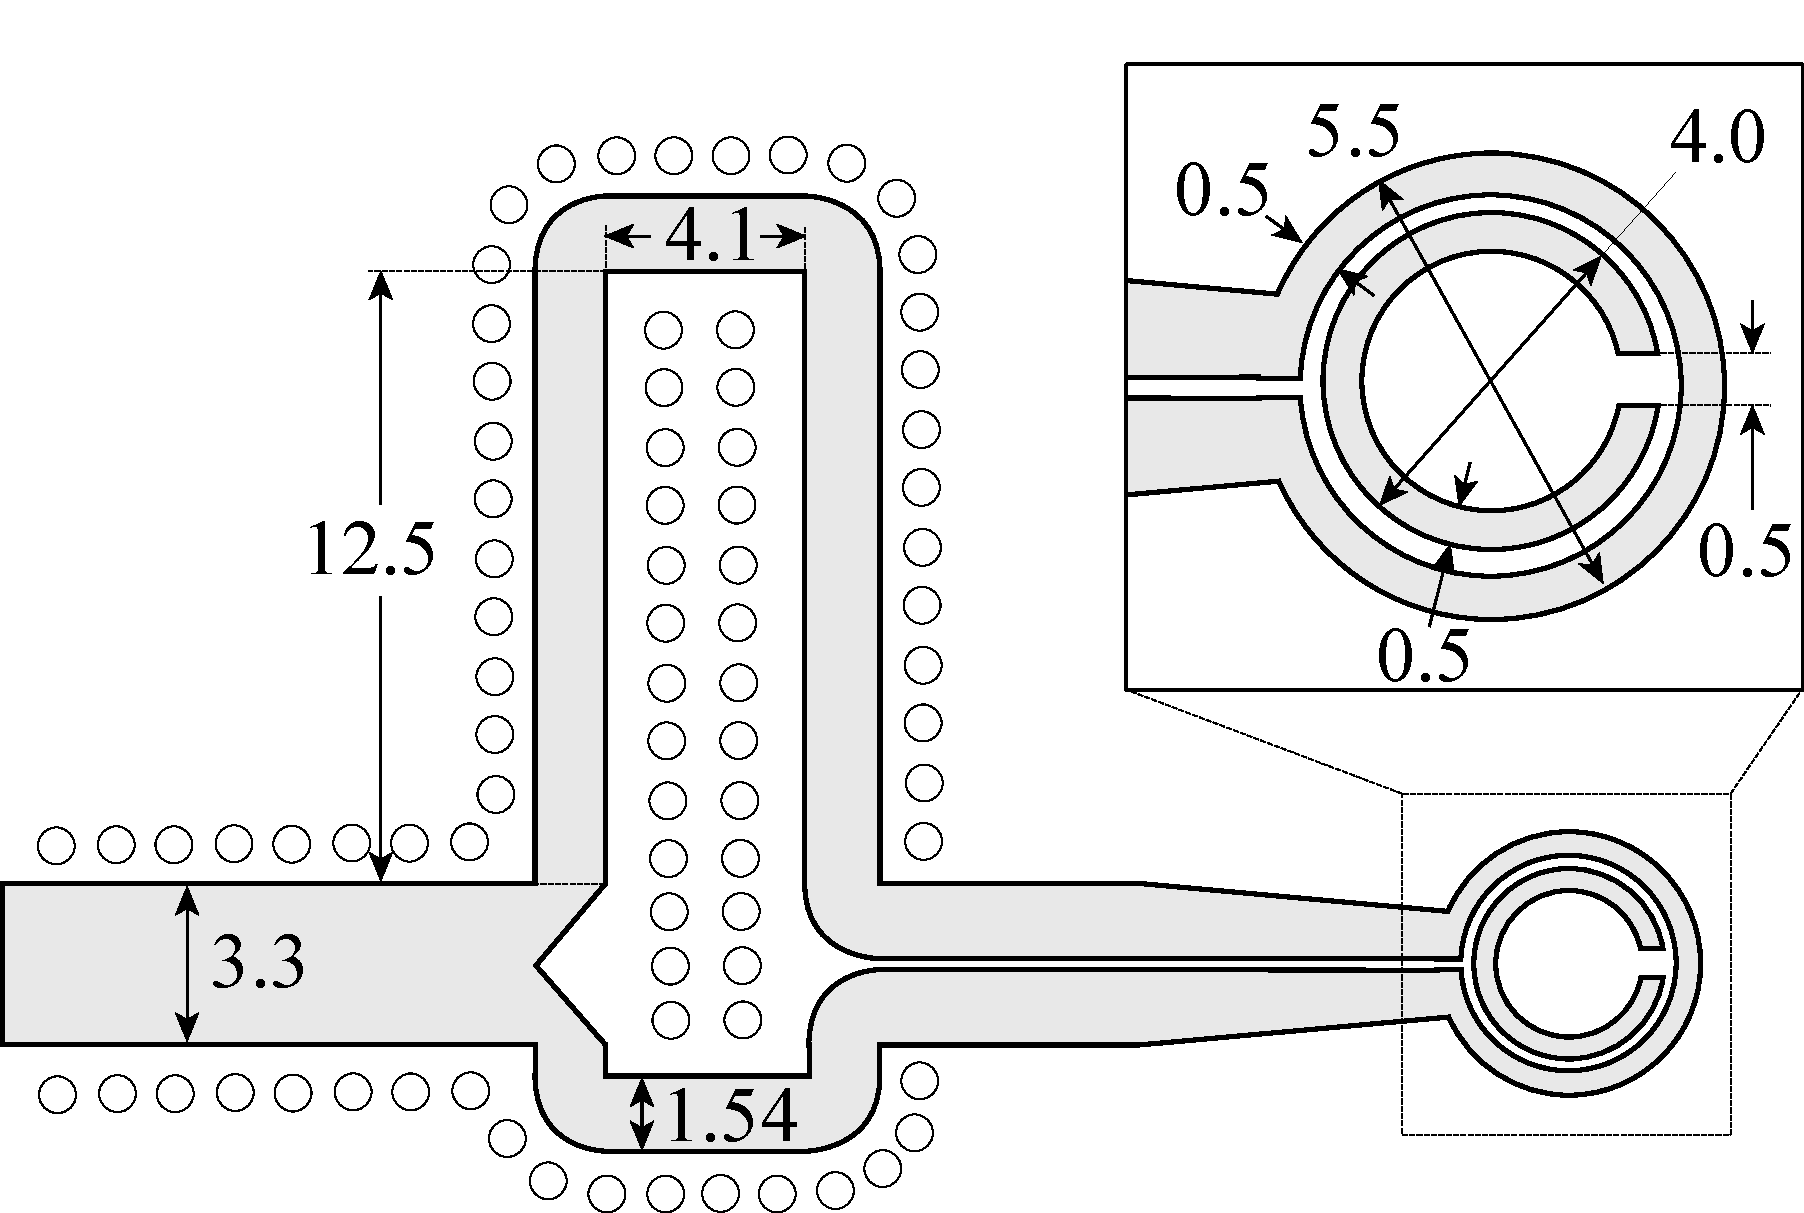
\includegraphics[scale = 0.45]{Exciter_Drawing.pdf}  
\caption{\textbf{Exciter board drawing} A feedline, 50:50 power splitter, and balun (\textbf{ba}lanced \textbf{un}balanced) feed the split ring resonator, which is coupled to the LGR. All dimensions are in mm. Optional mounting holes and radial access port for laser excitation are not shown}
\label{LGR_Exciter}
\end{figure}

Differential driving of the balun mitigates common-mode noise on the two traces, which might otherwise couple to the split-ring resonator. A via shield along a portion of the balun helps reduce interference and cross-talk between traces, controls trace impedance, and reduces radiative losses along the balun's $\pi$ phase delay arm. The exciter antenna is fabricated from a 1oz. copper trace with immersion silver finish on a 1.524 mm thick dielectric substrate (Rogers RO4350B). Although the proximity of the split-ring resonator perturbs the field distribution inside the LGR, both simulations and measurements suggest this effect is minimal and not the dominant source of inhomogeneity (See section \ref{field}).  

Although the microstrip balun is designed to match the feed-line and the split ring component of the exciter antenna at frequencies near 2.87 GHz, good matching is achieved from 2.5 GHz to 3.5 GHz as well. For drive frequencies between 2.5 and 3.5 GHz, the
exciter antenna board couples more than 90\% of incident MW power into the LGR, as shown in Figure \ref{LGR_tuning} (a). For a specific fixed frequency, the impedance matching may be further optimized by inserting a stub tuner between the MW source and the exciter antenna board, as shown in Figure \ref{LGR_tuning} (b). The stub tuner changes the effective electrical length of the exciter circuit and therefore modifies the coupling between the split ring resonator and the LGR. Similar matching can be achieved using a varactor diode instead of a stub tuner. 


\begin{figure}[t!]
\centering
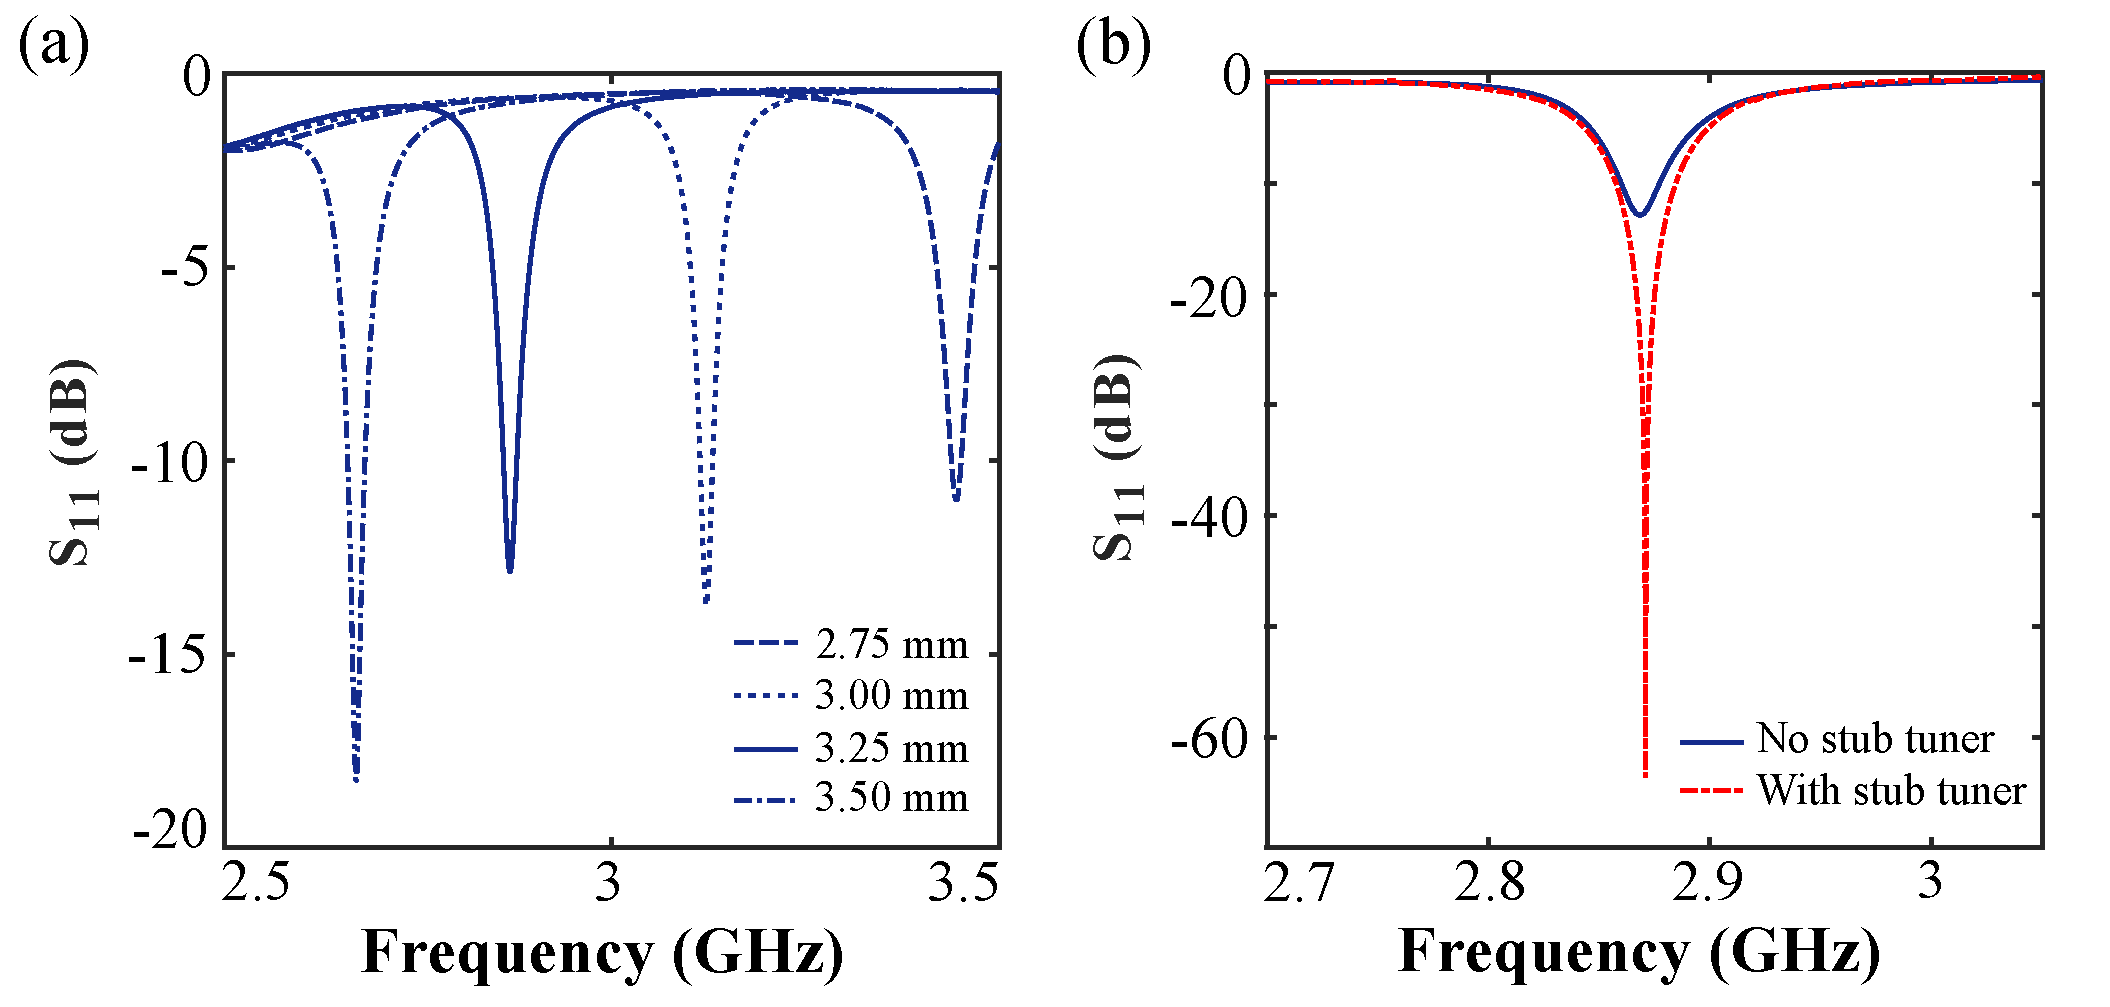
\includegraphics[width = \textwidth]{Figure_2.pdf}  
\caption{\textbf{Frequency tuning and impedance match-
ing of LGR composite device.} \textbf{(a)} The resonant frequency $f_0$ is adjusted by translating the sapphire shims in the four capacitive gaps. In the absence of a stub tuner, the LGR composite device exhibits $S_{11}$ values between -10 and -20 dB from 2.5 to 3.5 GHz, indicating at least $\gtrsim90\%$ of power delivered to the LGR composite device contributes to $B_1$ in this range. \textbf{(b)} Nearly perfect critical coupling can be achieved with
a stub tuner, allowing practically all incident MW power to contribute to $B_1$.}
\label{LGR_tuning}
\end{figure}

\pagebreak


%More robust coupling for implementable device

%Discussion of split ring exciter antenna and design outline of feedline and balun and design process of stepping through circuit etc.

%Talk about additional matching using stub tuner. 

%\begin{figure}[t!]
%\centering
%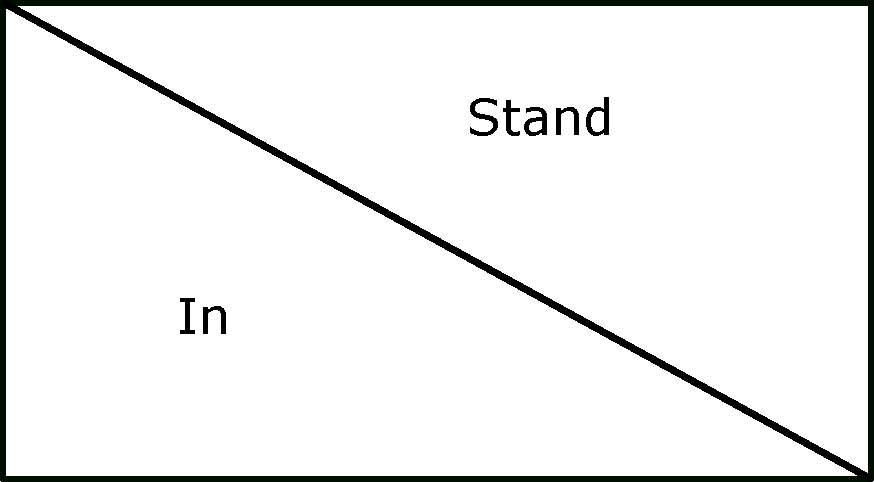
\includegraphics[width = \textwidth]{STANDIN.pdf}  
%\caption{\textbf{Eigenfrequency solution to LGR} \textbf{a)} \textcolor{red} {STANDIN. PLEASE REPLACE}}
%\label{LGR_Eigen}
%\end{figure}




\section{Electric Field}

One challenge that many MW solutions face is maintaining good coupling and a steady resonant frequency when a sample is introduced. For example, if a dielectric sample is placed on a planar resonator the dramatic change in capacitance between trace elements causes a shift in the resonant frequency \cite{bayat2014efficient, sasaki2016broadband, zhang2016microwave} of the oscillator. Just like planar fabricated resonators, the LGR is a lumped element device but its large size permits an improved spatial separation between the electric and magnetic fields in the cavity. The electric field in the TE\textsubscript{10} mode is confined to the capacitive gaps and thus has little interaction with a dielectric sample placed in the center cavity. In practice, fringing electric Fields from the capacitive gaps extend partially into the LGR's central loop as shown in Figure \ref{LGR_Electric}. However, at distances > 1 mm from the capacitive gaps, the electric Field magnitude |E| is decreased by >10x from the peak Field inside the capacitive gap. Consequently, insertion of a diamond (with
$\epsilon_r \approx 5.7$ at 3 GHz \cite{ibarra1997wide}) beyond this region has little if any effect on the LGR resonant frequency $f_0$.

\begin{figure}[t!]
\centering
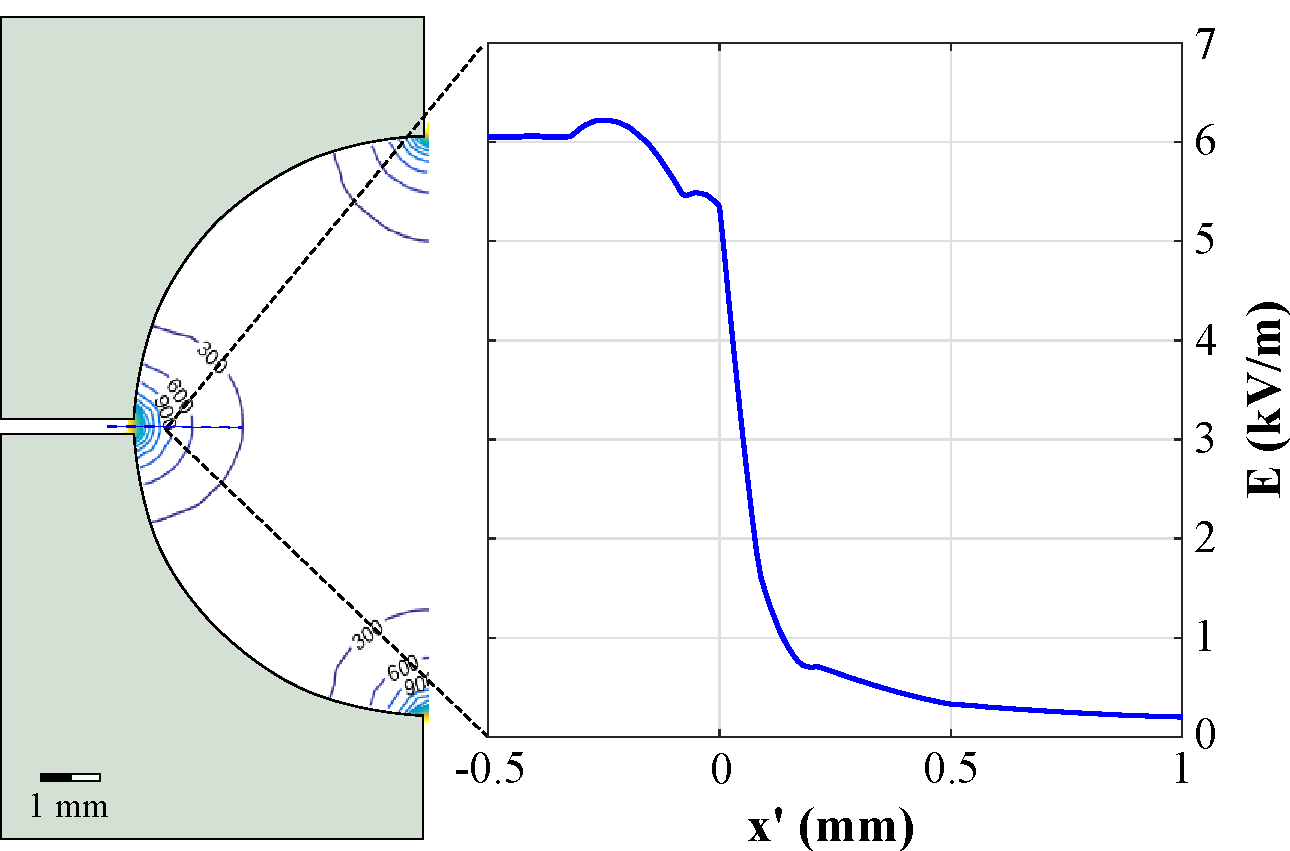
\includegraphics[scale = 0.55]{Figure_B_1.pdf}  
\caption{\textbf{Simulated electric field magnitude E in vicinity of LGR capacitive gap.} Inset depicts the electic field
magnitude E as a function of distance from the capacitive gap with $x' = 0$ mm corresponding to the plane of the central loop-gap interface.}
\label{LGR_Electric}
\end{figure}

%\begin{figure}[h!]
%\centering
%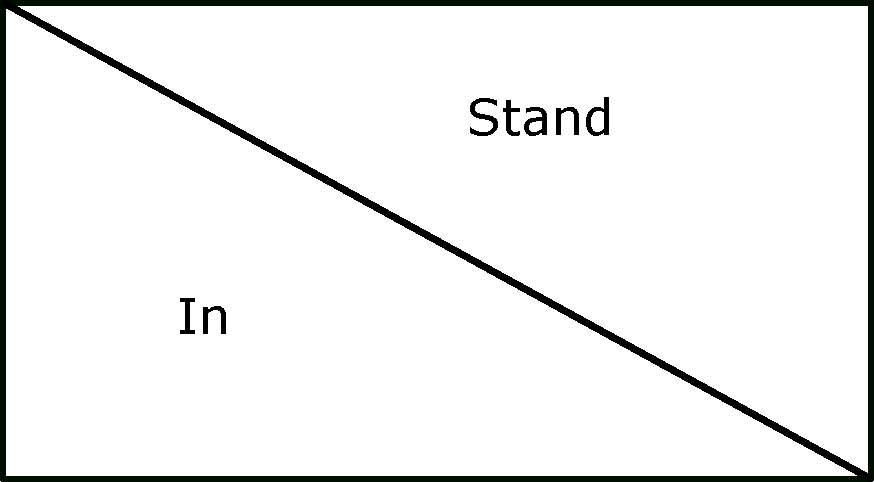
\includegraphics[width = \textwidth]{STANDIN.pdf}  
%\caption{\textbf{Electric field} \textbf{a)} \textcolor{red} {STANDIN. PLEASE REPLACE}}
%\label{LGR_Sample}
%\end{figure}


%% This is an example first chapter.  You should put chapter/appendix that you
%% write into a separate file, and add a line \include{yourfilename} to
%% main.tex, where `yourfilename.tex' is the name of the chapter/appendix file.
%% You can process specific files by typing their names in at the 
%% \files=
%% prompt when you run the file main.tex through LaTeX.

\chapter{LGR Performance and Field Characterization} \label{ch3}

In this chapter the LGR electrical and magnetic are discussed and measured. All simulations were completed in ANSYS HFSS a full-wave electromagnetic simulation tool. 

\section{Quality Factor}\label{quality}

As mentioned in section \ref{resonant_enhc}, The quality (or Q) factor of an oscillator quantifies how often (in terms of the oscillation period) the energy will oscillate back and forth until its initial amplitude is reduced by a factor of $1/e$. At critical coupling ($\beta = 1$) the intrinsic Q ($Q_0$) of the resonator (which quantifies the oscillation lifetime due to resistive losses) is calculated as the inverse of its fractional bandwidth ($FBW$),
\begin{equation}
Q_0 = \frac{1}{FBW} = \frac{f_0}{\Delta_{3dB}}.
\end{equation} 
The fractional bandwidth however is calculated from the loaded Q ($Q_L$) which takes into account coupling losses due to power reflection at the exciter antenna/LGR interface. Incorporating these reflections is achieved by assigning an external Q ($Q_e$) to account for these losses. $Q_e$ then combines with $Q_0$ in a parallel configuration
\begin{equation}
\frac{1}{Q_L} = \frac{1}{Q_0} + \frac{1}{Q_e},
\end{equation} 
to yield $Q_L$. The intrinsic Q, $Q_0$, and the external Q, $Q_e$, characterise the most dominant loss mechanisms of the device. Other loss mechanisms and their contribution to $Q_L$ are discussed in reference \cite{piasecki1993field}; they include, but are not limited to, loss in a sample, radiation losses, surface wave losses, hand-shaking (if not properly shielded), etc..

Since the quality factor is inversely proportional to the resonator bandwidth the LGR needs to exhibit fairly low Q in order to address all eight NV resonances and their shifts due to an external field. The LGR was thus designed to accommodate an NV ensemble that has been split using an up-to 14 gauss biasing field $B_0$. Since the NV gyromagnetic ratio ($\gamma_B$) is 2.8 MHz/gauss, this corresponds to an ideal bandwidth of 39 MHz and, at 2.87 GHz, a Q of $\sim$ 36. In addition to a wide dynamic range, a low Q allows for the use of concatenated pulse sequences without employing additional methods to evacuate power from the resonator before the next pulse is applied (e.g. active cancellation). 

\subsection{Ringdown time}

As mentioned above, in order to apply concatenated MW pulses to a sample in the LGR (as is done often in NMR and NV applications \cite{}) the power oscillating in the cavity must be evacuated or dissipated in between pulses. One method used is to apply active cancellation techniques that either introduce extra components to the excitation circuitry to abruptly de-tune the resonator before the next pulse is applied  \cite{} or apply a secondary pulse that is designed to destructively interfere with the cavity ring-down \cite{Franck2015Active}. Another, and also the technique applied here, is to make the resonator intrinsically lossy and therefore dissipate the left-over power in the cavity as either heat or radiation. To calculate the ring-down time $\tau_{ring}$ of the LGR we apply a damping exponential to the field within the cavity such that $B(t) = B_{init}e^{-\pi f_0t/Q}$ (neglecting any phase caused by a shift in the resonant frequency), and solving for the time $t$ at which the amplitude has decreased to $1/e \cdot B_{init}$. Doing this yields
\begin{equation}\label{eqn33}
\tau_{ring} = \frac{Q}{\pi f_0}.
\end{equation} 
Using equation \ref{eqn33} and the bandwidth and center frequency extracted from the measured data in Figure \ref{LGR_tuning}, one calculates $\tau_{ring} = 4$ ns which is sufficient for standard NV and NMR pulsed protocols \cite{Smeltzer2009Robust,Jelezko2004Observation,Steiner2010Universal}.

\section{Simulating the Magnetic Field}

The $B_1$ field distribution in the center loop of the LGR was simulated using the full-wave electromagnetics simulation suite ANSYS HFSS. The simulation includes the 200 $\upmu$m dielectric shims and the full exciter circuit depicted in Figures \ref{LGR_Exciter} and \ref{LGR_drawing}. The solution type was set to "driven modal" since the exciter board has a single trace interconnect and thus requires the solution of TE and TM propagation modes. Figure \ref{LGR_simulated} shows the $B_1$ distribution computed by HFSS at an input power of 42 dBm. The exciter board (which extends over the LGR center loop along the line $x = y$ in the figure) clearly imparts a small perturbation on the otherwise radially symmetric field. The simulation predicts $B_1 \approx 4.8$ gauss at the LGR center and a maximum field of $B_1 \approx 5.4$ gauss at the perimeter. Two metrics are used to quantitatively characterize 2D regions of homogeneity , the fractional root-mean-square inhomogeneity $\sigma_{rms}$ calculated as 
\begin{equation}\label{sigma_rms}
\sigma_{rms} = \sqrt{\frac{\Sigma_{i = 1}^N(B_{1,i}-B_{2,i})^2}{N}} \cdot \mu_N^{-1},
\end{equation}
where $i$ is an index over all $B_1$ field values in the region, $N$ is the total number of values, and $\mu_N$ is the mean of all $N$ values, and the fractional peak-to-peak variation $\sigma_{pp}$ calculated as
\begin{equation}\label{sigma_pp}
\sigma_{pp} = \frac{\left[B_1^{max} - B_1^{min}\right]}{\mu_N}.
\end{equation} 
The use of both metrics facilitates comparison with alternative existing designs. Within a 32 mm\textsuperscript{2} circular area centered in the LGR central loop, simulations indicate $\sigma_{rms} = 3.8\%$ and $\sigma_{pp} = 11\%$, whereas in a smaller 11 mm\textsuperscript{2} circular area, simulations indicate $\sigma_{rms} = 1\%$ and $\sigma_{pp} = 2\%$.

\begin{figure}[t!]
\centering
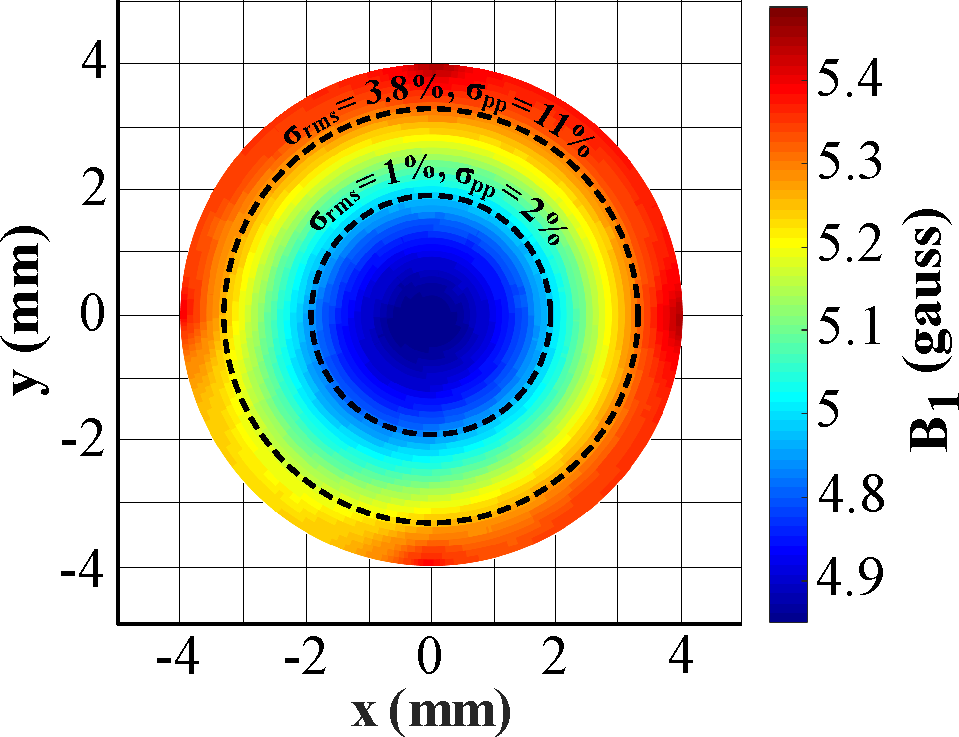
\includegraphics[scale = 0.6]{FieldSimulation.pdf}  
\caption{\textbf{Simulated magnetic field} Top-down cross section of center loop of LGR. Slice is taken at half height h. Simulations suggest the $B_1$ field distribution
should be approximately radially symmetric, with the leading order deviation resulting from the exciter antenna. Dashed lines indicate the 32 mm\textsuperscript{2} and 11mm\textsuperscript{2} areas within which the $B_1$ field uniformity is evaluated.}
\label{LGR_simulated}
\end{figure}

As a three dimensional cavity resonator, the LGR provides better axial field uniformity than planar-only geometries \cite{floch2016towards,kapitanova2017dielectric,angerer2016collective}. Figure \ref{LGR_axial_simulated} plots the simulated $B_1$ along the LGR's symmetry axis, illustrating the improved axial field uniformity possible with three-dimensional cavity
resonators, compared to that of planar-only geometries. The presence of the split ring resonator at $z = 4.024$ mm perturbs $B_1$ inside the LGR, shifting the point of maximal $B_1$ down by 0.4 mm, away from the split-ring resonator. Within a cylindrical volume of 3.14 mm\textsuperscript{3} (1 mm radius and 1 mm thickness), centered around the point of maximal $B_1$, the simulations predicts $\sigma_{rms} = 0.78\%$ and $\sigma_{pp} = 3.7\%$. For a larger cylindrical volume of 12.6 mm\textsuperscript{3} (2 mm radius and 1 mm thickness), the simulation predicts $\sigma_{rms} = 2\%$ and $\sigma_{pp} = 8\%$. These dimensions are comparable to those of commercially available single-crystal diamonds. Additionally, Figure \ref{LGR_axial_simulated} gives 1D regions of homogeneity along the LGR symmetry axis.

\begin{figure}[t!]
\centering
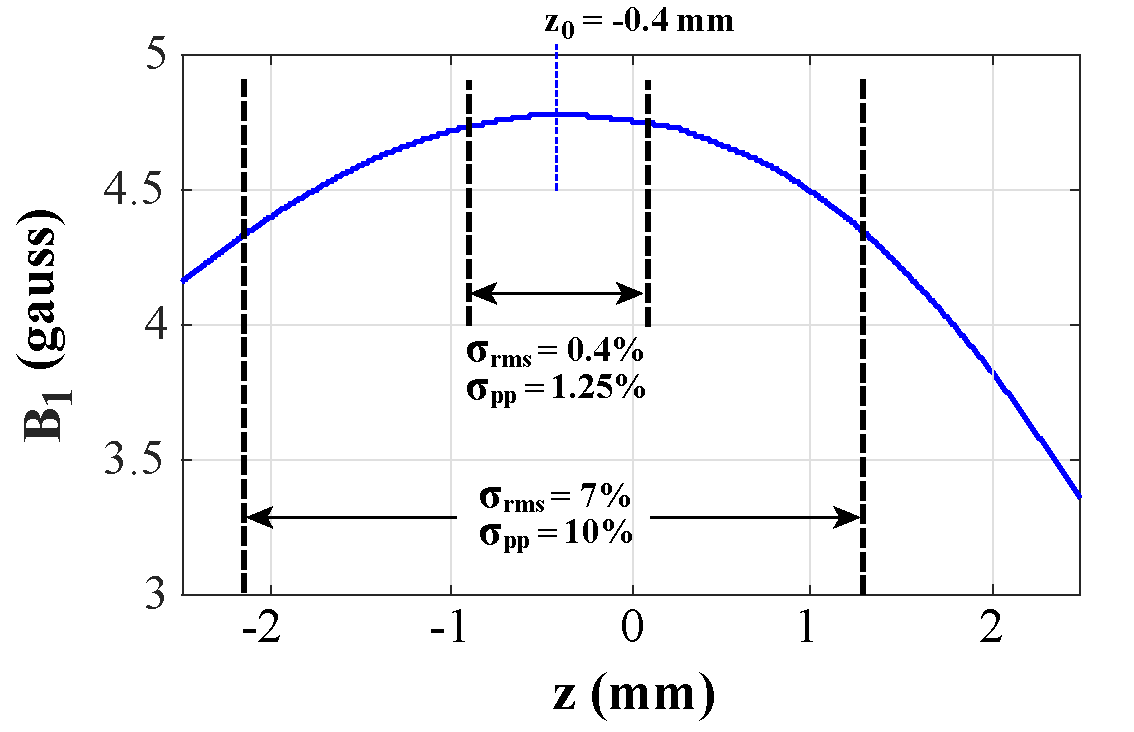
\includegraphics[scale = 0.6]{Figure_B_2.pdf}  
\caption{\textbf{Simulated $B_1$ field along LGR symmetry axis.} The symmetry plane of the LGR is located at $z = 0$ mm. The edges of the LGR are at $z = \pm 2.5$ mm, and the split-ring resonator is located at $z = 4.024$ mm. The presence of the split-ring resonator shifts the point of maximal $B_1$ off-center to $z_0 = -0.4$ mm.}
\label{LGR_axial_simulated}
\end{figure}

\section{Measuring the Magnetic Field} \label{field}

Measuring the magnetic field distribution within the central loop of the LGR can be done in several ways. The simplest is to raster scan a magnetic probe across the cross section one wants to measure. However there are many drawbacks to this method. First, the spatial resolution is set by the size of the probe tip. Figure \ref{LGR_probe} shows the normalized magnetic field distribution of the LGR, measured by a 100B Beehive magnetic probe. The shielded loop diameter of the probe is 1 mm and thus the resolution is poor. Second, the probe has very little access to the center of the cavity. The data in Figure \ref{LGR_probe} was, for example, taken 1 mm above the LGR center loop; a region in which the magnetic field is highly divergent. Since the magnetic loop only measures the component of the field that lies parallel with its cental axis this provides a limited picture of the total field distribution. Third and finally, the proximity of the probe to the LGR perturbs the field and thus the distribution measured is an altered version of the unperturbed scenario. 

Another method--with similar drawbacks--is to measure the cavity transmission characteristics under intentional perturbation by a metal probe tip. by moving the perturbing probe tip, the transmission parameter $S_{21}$ (when an out-coupler loop is placed into one of the lateral loops) changes proportional to the field at the point of measurement. Thus, if the metal tip is scanned across the cavity, a picture of the field distribution can be extracted.  

\textcolor{red}{Since the LGR in this thesis is designed to supply MWs to NV centers, one can utilize the NV centers in turn to measure the strength of the supplied MWs}. If the period of the Rabi frequency (as described in section \ref{Rabi}) can be determined, then one can, using a simple relation, calculate the magnitude of $B_1$. This measurement of the field does not suffer from the drawbacks of the other two mentioned above and thus, it's the method employed in this thesis. The following subsections describe the measurement apparatus, measurement process, and calculations used to infer the strength of the $B_1$ field at various points within the LGR center loop.

\begin{figure}[t!]
\centering
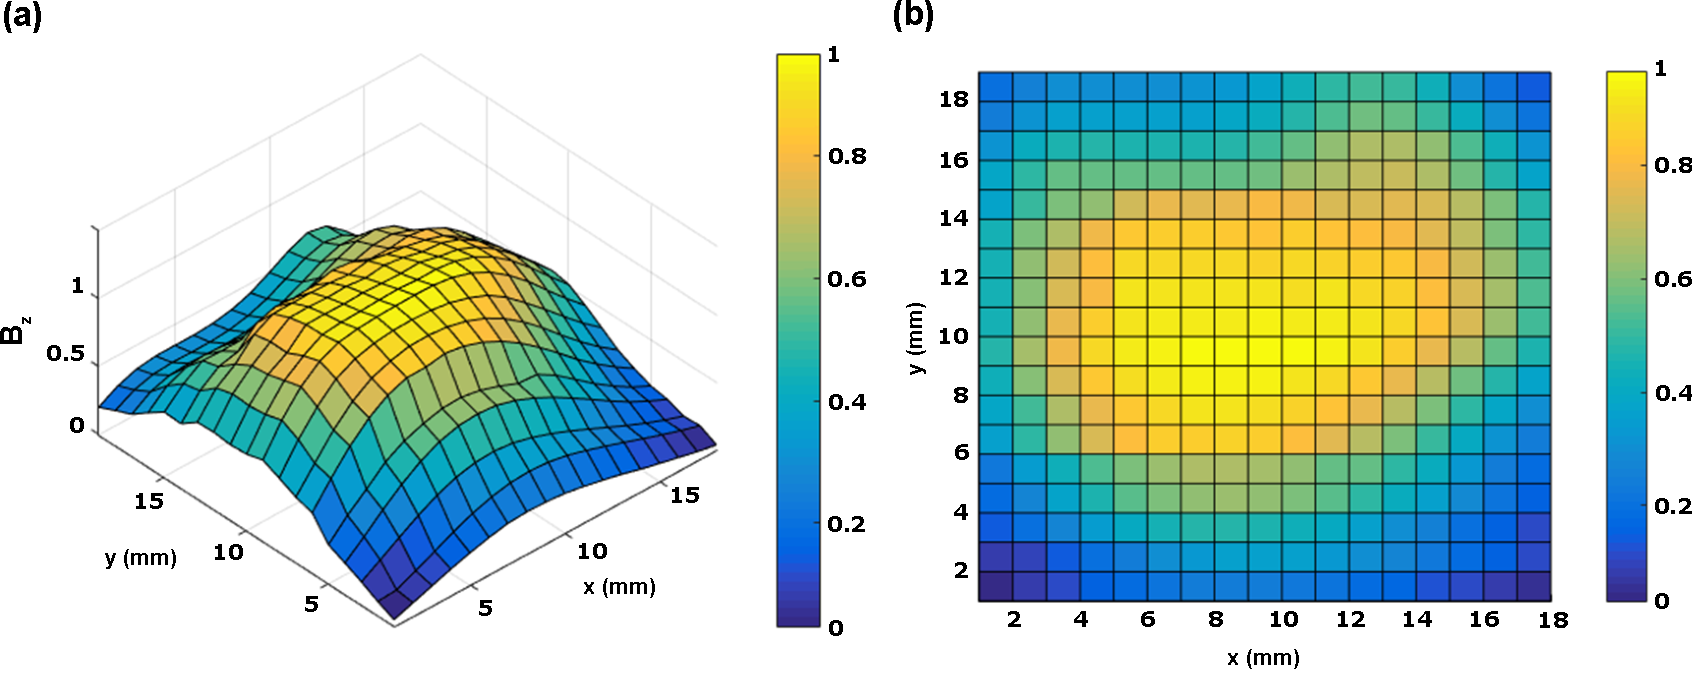
\includegraphics[width = \textwidth]{probefield.pdf}  
\caption{\textbf{$B_z$ component of field measured with probe} \textbf{a)} 3D surface plot of $B_z$ field distribution using a Beehive 100B magnetic field probe. Color bar units are normalized magnetic field. Normalized to their maximum value. \textbf{b)} Same data as in a) but top-down view. }
\label{LGR_probe}
\end{figure}

\subsection{Experimental setup} \label{setup}

\begin{figure}[b!]
\centering
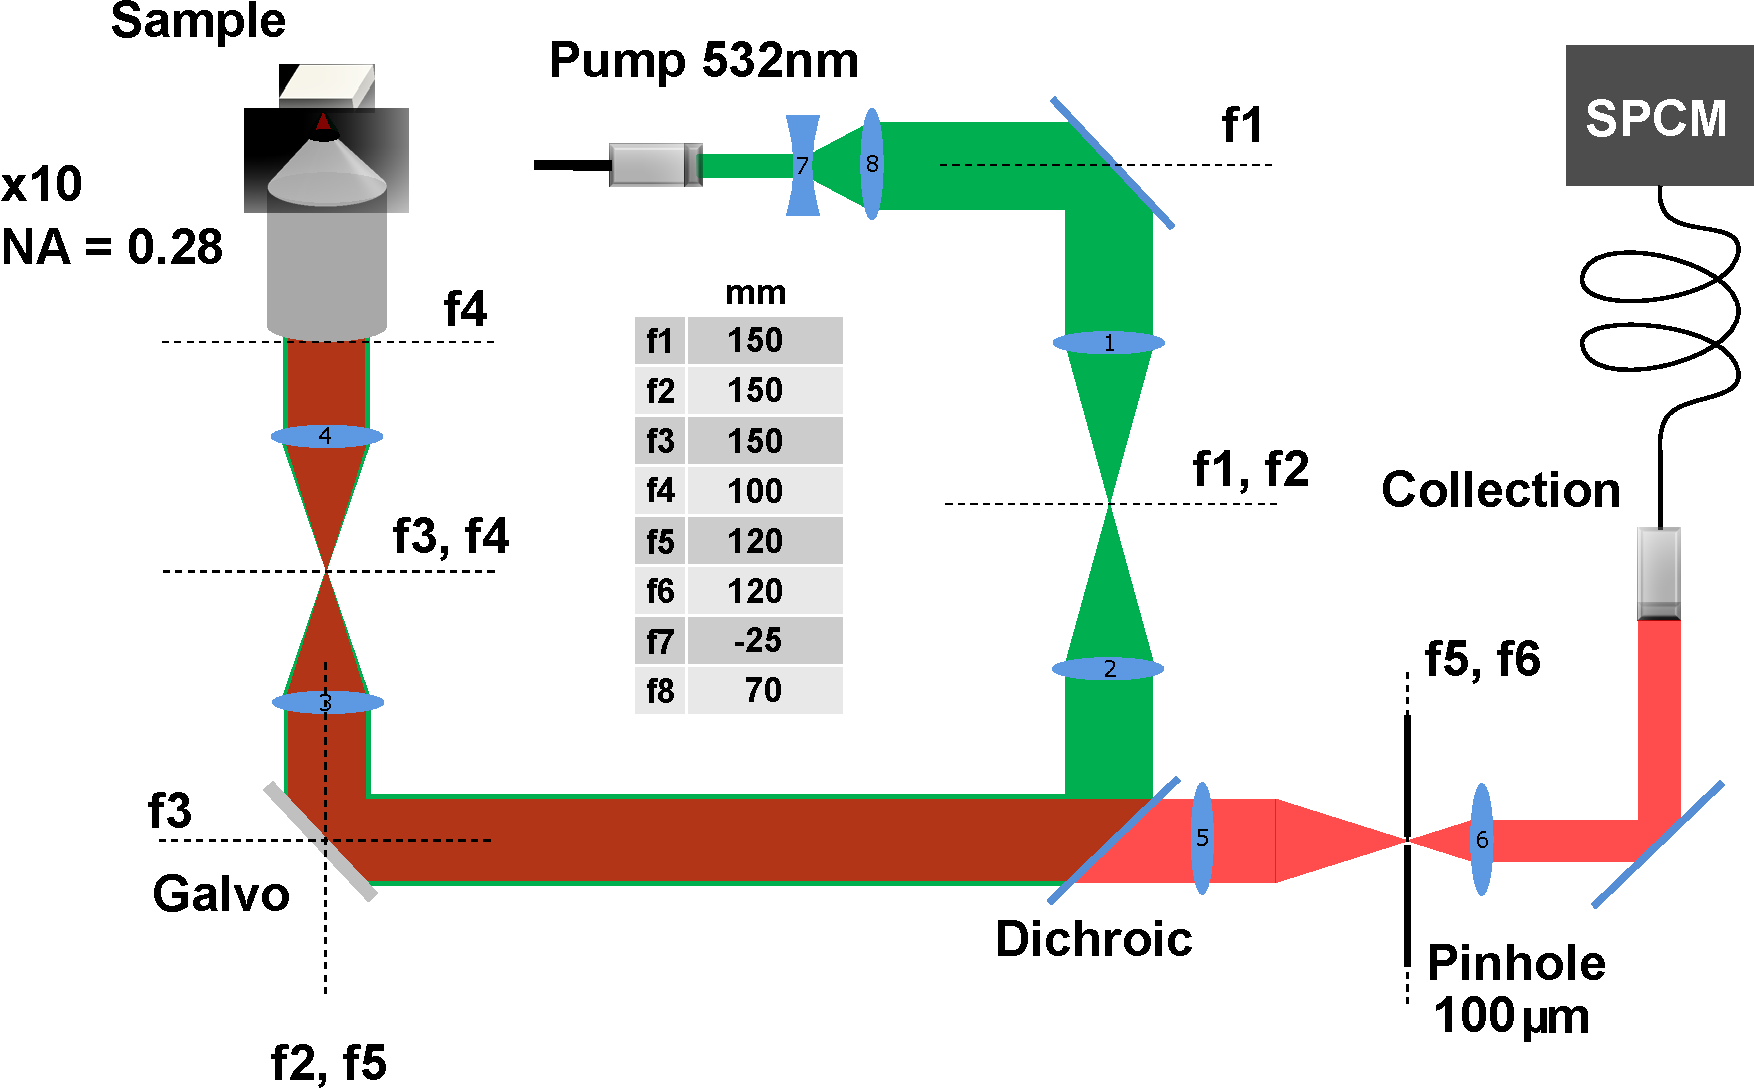
\includegraphics[scale = 0.1]{Confocal_Diagram_001.pdf}  
\caption{\textbf{Confocal Microscope} Custom built confocal microscope used to measure $B_1$ in LGR.}
\label{LGR_confocal_image}
\end{figure}

To measure the field distribution within the LGR center loop a home-built scanning confocal microscope [Figure \ref{LGR_confocal_image}] was employed. The confocal microscope supplies the 532 nm pump beam to polarize the NVs and collects the resulting fluorescence using a dichroic beam splitter and a single photon counting module (SPCM). The three main sections of the experimental setup are the pump path, the collection path, and the sample path. The pump path [Figure \ref{LGR_confocal} (a)] includes all optics from the launch of the excitation beam to the dichroic. Optical pulsing is accomplished using an acousto-optic modulator (AOM) that is located before the fiber launch; Ie. the laser passes through an AOM and is then coupled into a single mode (SM) polarization maintaining fiber which is then launched as the pump beam. The SM fiber picks off the first order refracted beam of the AOM and rejects the rest so no iris needed. The pump path contains a fiber launch (FiberPort coupler PAF-X-11-B), a half wave plate to selectively excite and address NV orientations, a beam expander consisting of a positive and negative focal length lens, and a 1:1 telescope. The 1:1 telescope (ie. no magnification) serves to change the angle of the beam down the sample path without moving the excitation spot off the galvo mirrors. In order for this to happen, the distance between the center of the two galvo mirrors and the last lens of the telescope must be equal to the focal length of the lens. In this way the angle of the beam into the objective can be changed without needing to reposition the galvos---which is a function designed for convenience only. The beam expander changes the collimation of 532 nm into the objective and therefore changes where the green comes into focus along the optical axis of the objective. This effectively serves to overlap the green excitation and the red fluorescence. Overlapping the two beams serves to maximize collection through the pinhole on the collection arm since the pinhole is initially aligned using the back-reflected green pump laser.

\begin{figure}[t!]
\centering
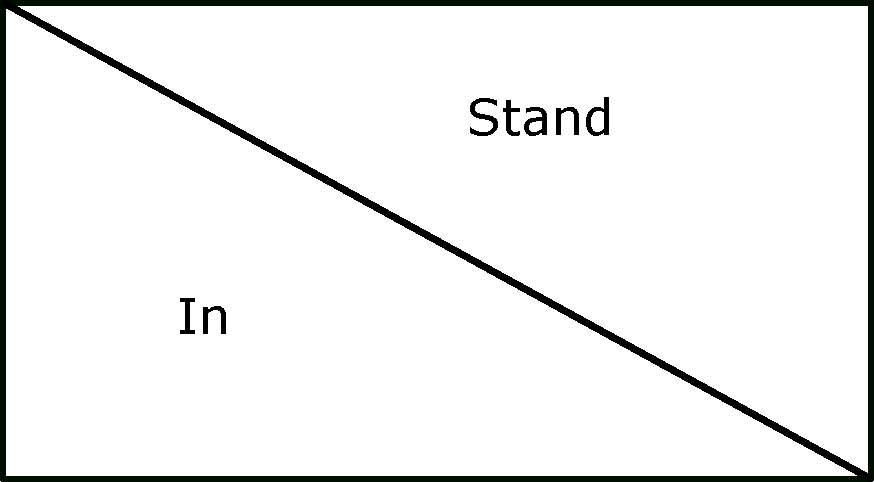
\includegraphics[scale = 0.8]{STANDIN.pdf}  
\caption{\textbf{STANDIN for Confocal Diagram} Confocal DIAGRAM STANDIN}
\label{LGR_confocal}
\end{figure}

The collection path (or arm) [Figure \ref{LGR_confocal} (b)] begins at the dichroic and ends at the collection end through a multimode fiber (65 $\upmu$m core) and into the SPCM. The path consists of the dichroic, a pinhole between two telescoping lenses, a multimode fiber, and an SPCM. The dichroic (Semrock Brightline FF552-Di02-25x36) filters the green pump beam from the sample fluorescence by reflecting wavelengths below 552nm and transmitting everything above. The first lens of the telescope focuses the beam down and passes it through a pinhole that spatially filters the image in X and Y to provide improved resolution. The pinhole was chosen to be 100 $\upmu$m to maximize collection while sacrificing some lateral resolution in the image. Generally the pinhole diameter ($p_d$) should be selected using the following equation:
\begin{equation}
p_d = \frac{1.22 \lambda}{NA} \cdot M_{objective} \cdot M_{telescope} 
\end{equation}
The telescope in the sample path de-magnifies the beam by a factor $M_{telescope} = \frac{100}{150} = 0.67$ which is the ratio of the focal lengths of the lenses in the sample path. The objective used has a magnification of x10 which leads to a nominal pinhole size of 20 $\upmu$m. However, this limits the amount of fluorescence collected because the pinhole filters out-of-focal-plane light which constitutes a large part of the signal. Since measuring the $B_1$ field distribution in the LGR center cavity does not require high spatial resolution, a 100 $\upmu$m diameter pinhole was chosen such that each measurement wasn't fluorescence starved. The filtered beam then passes through a second lens which focuses it onto the core of a multimode fiber connected to the SPCM. The multimode fiber allows for some rejection of ambient light without too much loss of the fluorescence signal. To further minimize the collection of ambient light, the multimode fiber dock and SPCM are enclosed in a light tight box. 

The sample path [Figure \ref{LGR_confocal} (c)] also begins at the dichroic, but passes through the galvanometer and objective and ends at the sample within the LGR center loop. It consists of a galvanometer, a 4F lens system (telescope), an iris, an objective and a sample stage. The objective used (Mitutoyo 378-803-3, M Plan Apo 10x $NA=0.28$) has a long working distance of 34 mm. The long working distance was necessary to minimize perturbations of the $B_1$ field by the metal housing of the objective. Future NV wide-field imaging applications may require ceramic-tipped objectives. Finally, although this microscope has a galvanometer capable of scanning the beam over an area of $\sim$ 250 $\upmu$m x 250 $\upmu$m the beam was held steady and the resonator moved to ensure $B_0$ is consistent for all measurements across the central loop of the LGR.


\subsection{Measurement process}

The strength and homogeneity of $B_1$ within the LGR central loop is evaluated employing standard NV techniques, as described in detail if references \cite{pham2013magnetic,childressthesis2011coherent,mazethesis2010quantum}. More specifically, a custom built scanning confocal microscope (as described in section \ref{setup}) measures the Rabi nutation frequency $\Omega_R$ of an ensemble of NV centers. A $\{$100$\}$-cut diamond plate containing $\sim 1 \times 10^{14}$ NV/cm$^3$ is mounted at the center of the LGR with the $<$100$>$ crystallographic axis collinear with the LGR axis. A rare earth magnet creates a static magnetic bias field $B_0$, which shifts the energies of the $m_s=\pm1$ ground-state Zeeman sublevels. The energy shifts are given to first order by~\cite{taylor2008high}
\begin{equation}
\Delta E \approx \text{g}_{\text{s}} \upmu_\text{B} m_s \vec{B}_0\cdot \hat{n}_i,
\end{equation}
where $\hat{n}_i$ denotes a unit vector oriented along one of the four diamond crystallographic axes. By judicious choice of $\vec{B}_0$, all eight energy levels and associated $m_s\!=\!0\! \leftrightarrow \!m_s\! =\!\pm1$ magnetic dipole transitions can be isolated as shown in Fig. \ref{LGR_Rabi_meas}(a). The resonator is tuned to excite a single NV transition, yielding Rabi oscillations [Fig. \ref{LGR_Rabi_meas}(b)]. The data is fit to an exponentially decaying sinusoid in order to extract the Rabi frequency $\Omega_R$, from which the magnitude of $B_1$ can be calculated (discussed below in section \ref{calcRabi}). 

\begin{figure}[t!]
\centering
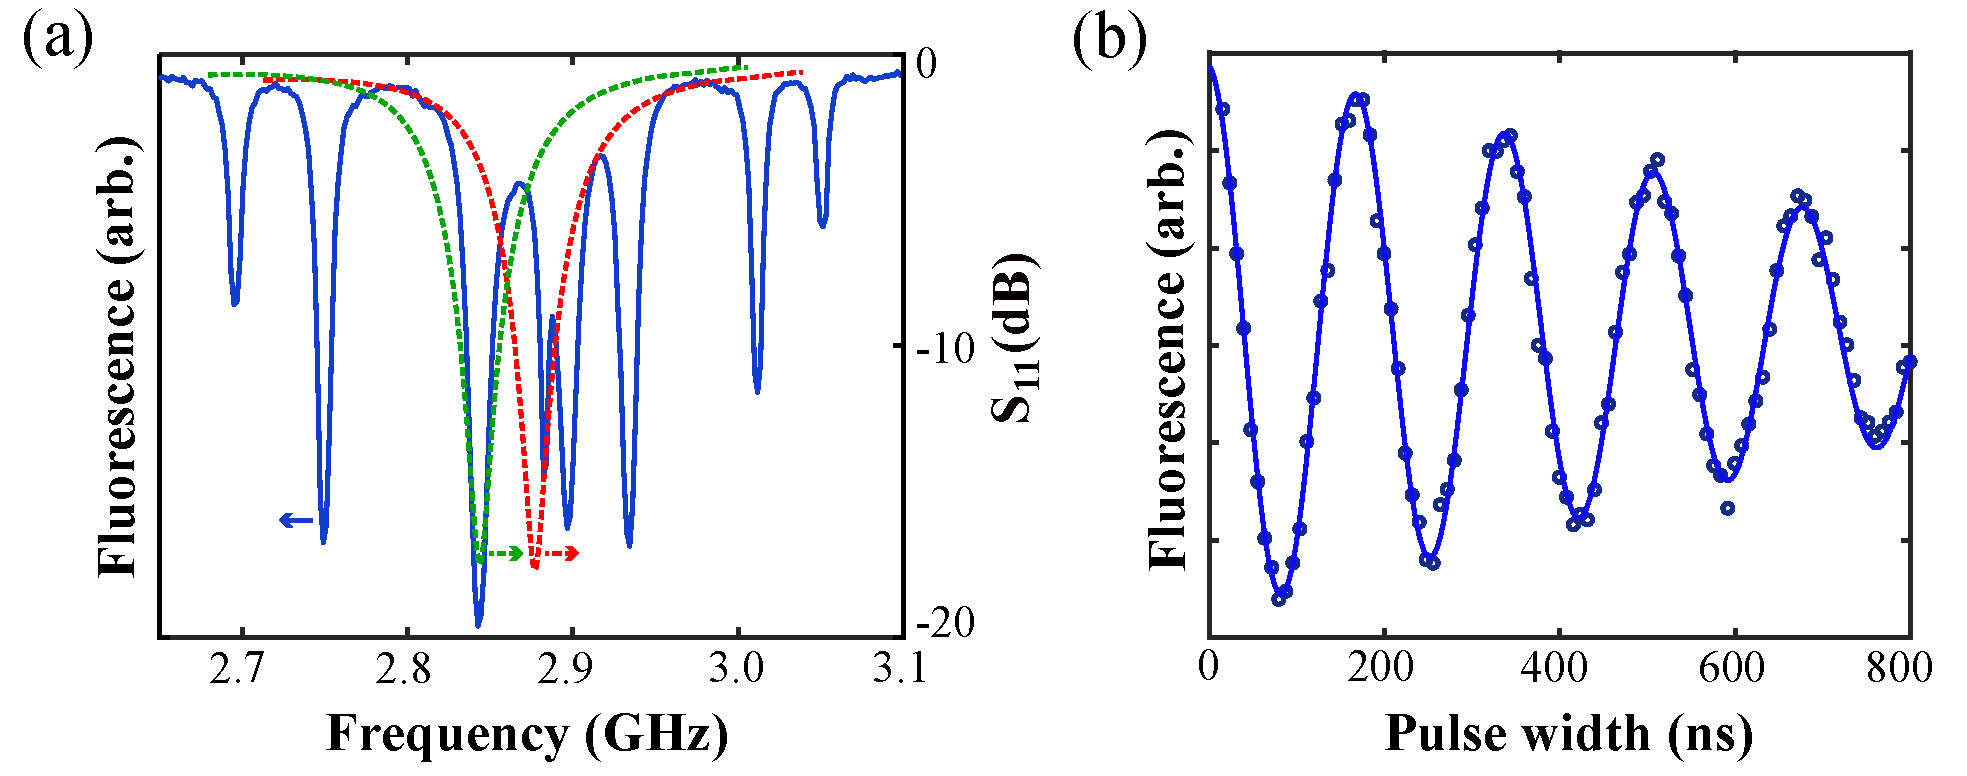
\includegraphics[scale = 0.45]{Figure_3.pdf}  
\caption{\textbf{LGR driving of an NV ensemble} \textbf{(a)} NV electron spin resonance spectrum (\textcolor{blue}{\textbf{---}}) under application of bias field $B_0$. The bias field allows individual addressing of all eight NV resonances, arising from the combination of the two allowed magnetic dipole transitions with the four possible NV orientations. The NV hyperfine structure is obscured by MW power broadening and the contrast variation between the NV resonances is attributed primarily to the $S_{11}$ line-shape. The $S_{11}$ parameter is shown before (\textcolor{red}{\textbf{-\,-\,-}}) and after (\textcolor{dolla-bill}{\textbf{-\,-\,-}}) shifting the LGR resonant frequency $f_0$ to the target NV resonance. Arrows indicate corresponding y axes. \textbf{(b)} Typical data depicting Rabi oscillations under MW excitation at the target NV resonance frequency indicated in (a). Data (\textcolor{navyblue}{$\mathbf{\circ}$}) is fit (\textcolor{blue}{\textbf{---}}) to an exponentially decaying sinusoid.}
\label{LGR_Rabi_meas}
\end{figure}

In this geometry, the $B_1$ field is oriented along the [100] crystallographic axis of the diamond, degenerately offset from all four NV axis orientations by half the tetrahedral bond angle $\theta_{\text{tet}}/2 = \text{ArcCos}\frac{1}{\sqrt{3}} \approx 54^\circ$. NV Rabi oscillations are driven by the $B_1$ field component transverse to the NV symmetry axis, reducing the Rabi frequency by $\sqrt{2/3}$ \cite{sasaki2016broadband}. To ensure $\vec{B}_0$ is consistent for all measurements across the LGR central loop, the confocal excitation volume is held fixed with respect to the $B_0$-generating permanent magnet, and the diamond and LGR composite device are translated together. The process is then repeated at a locus of points within the LGR center loop (discussed below in section \ref{LGRfield}).

%A static magnetic field ($B_0$) is applied to split the NV resonances and the sapphire shims (tuning process described in section \ref{tuning} are adjusted to tune the resonator to a single NV resonance as shown in Figure \ref{LGR_Rabi_meas} (a). A long working distance objective collects the NV fluorescence while its 34 mm working distance mitigates the effect of the metal objective housing on $B_1$. To measure $\Omega_R$ the NVs within the confocal volume are consecutively polarized, driven, and read out while sweeping the pulse length of the MW driving field. Using a gated single photon counting module, the fluorescence is collected and plotted against the MW pulse length

% Talk about experiment taking Rabi data, ie. Rabi pulse sequence, moving resonator, checking ESR, choosing ESR etc.

\subsection{$B_1$ from Rabi} \label{calcRabi}

calculating $B_1$ from Rabi frequency using rotating wave approx. etc, essentially where sqrt(3) comes from.

\section{LGR field distribution} \label{LGRfield}

The actual measured field distribution

\begin{figure}[t!]
\centering
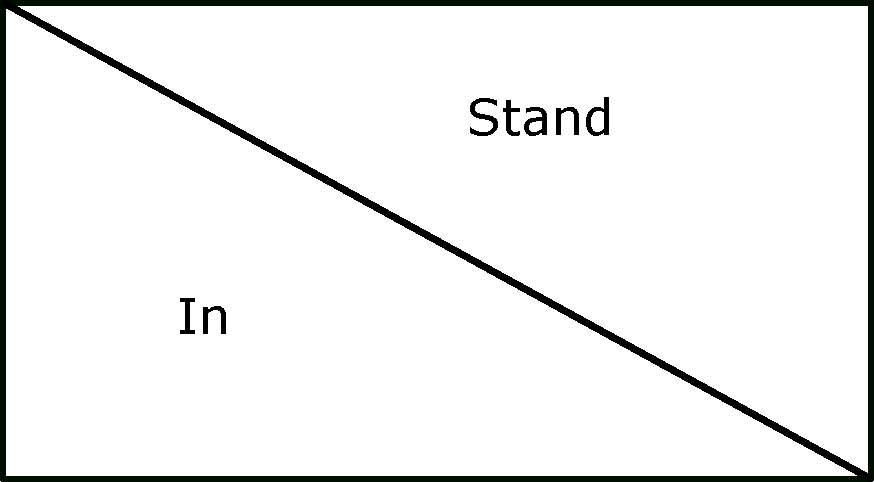
\includegraphics[scale = 0.8]{STANDIN.pdf}  
\caption{\textbf{STANDIN for Field} Field STANDIN}
\label{LGR_confocal}
\end{figure}




\appendix
\chapter{Tables}

\begin{table}
\caption{Armadillos}
\label{arm:table}
\begin{center}
\begin{tabular}{||l|l||}\hline
Armadillos & are \\\hline
our	   & friends \\\hline
\end{tabular}
\end{center}
\end{table}

\clearpage
\newpage

\chapter{Figures}

\vspace*{-3in}

\begin{figure}
\vspace{2.4in}
\caption{Armadillo slaying lawyer.}
\label{arm:fig1}
\end{figure}
\clearpage
\newpage

\begin{figure}
\vspace{2.4in}
\caption{Armadillo eradicating national debt.}
\label{arm:fig2}
\end{figure}
\clearpage
\newpage

%% This defines the bibliography file (main.bib) and the bibliography style.
%% If you want to create a bibliography file by hand, change the contents of
%% this file to a `thebibliography' environment.  For more information 
%% see section 4.3 of the LaTeX manual.
\begin{singlespace}
\bibliography{References_Library_Proposal}
\bibliographystyle{plain}
\end{singlespace}

\end{document}

